\documentclass[conference]{IEEEtran}
\IEEEoverridecommandlockouts
\renewcommand{\ttdefault}{cmtt}
\usepackage{cite}
\usepackage{amsmath,amssymb}
\usepackage{graphicx}
\usepackage{booktabs}
\usepackage{multirow}
\usepackage{array}
\usepackage{xcolor}
\usepackage{textcomp}
\usepackage{url}
\usepackage{balance}
\usepackage{microtype}
\usepackage{tikz}
\usetikzlibrary{positioning,arrows.meta,calc,fit,shapes.misc,decorations.pathreplacing}
\usepackage[hidelinks]{hyperref}
\usepackage{listings}

\DeclareRobustCommand{\code}[1]{\texttt{\detokenize{#1}}}
\newcommand{\LAT}{\ensuremath{L}}
\def\BibTeX{{\rm B\kern-.05em{\sc i\kern-.025em b}\kern-.08em T\kern-.1667em\lower.7ex\hbox{E}\kern-.125em X}}
\emergencystretch=2em
\graphicspath{{figures/}}

\lstset{basicstyle=\ttfamily\scriptsize,frame=single,numbers=left,numberstyle=\tiny,
  keywordstyle=\bfseries,columns=fullflexible,breaklines=true,xleftmargin=1.5em,
  language=Verilog,morekeywords={assign,always,posedge,case,endcase,wire,reg,localparam,module,endmodule}}

\begin{document}

\title{Design, Verification and Interactive Waveform Analysis of a\\Direct-Mapped Cache Controller}

\author{\IEEEauthorblockN{Author Name}
\IEEEauthorblockA{Modern Computer Architecture (MCA) Capstone Project\\
Department of Computer Science\\
Software-only implementation: Verilog, Icarus Verilog, Yosys, Python}}

\maketitle

\begin{abstract}
Main memory is much slower than a processor, so a cache is used to keep recently used blocks close to the core. This report describes the complete design, verification and analysis of a synthesizable direct-mapped cache controller: a 1~KB cache with 16-byte blocks and 64 lines, a six-state finite-state machine (FSM), a block-oriented memory interface with configurable latency, and a self-checking testbench with an independent reference model. We explain every cache term used, derive the address mapping and the timing equations, and show how each equation appears in simulation waveforms. The read-only controller passes eleven directed and randomized tests at five memory latencies; thirteen deliberately injected design bugs were used to check the testbench, and twelve were detected (the thirteenth is behaviorally equivalent). Measured hit time is 2 cycles and the miss penalty is $L+5$ cycles for a memory latency of $L$ cycles. Across five workloads the hit rate ranges from 99.8\% (repeated access) to 0\% (conflicting addresses), and the measured average memory access time (AMAT) matches the analytical formula exactly. A synthesis estimate with Yosys gives 635 four-input look-up tables, 487 flip-flops and 18 block RAMs in an FPGA-style mapping. Finally, a local web portal runs the real Icarus Verilog simulation and shows the resulting Value Change Dump (VCD) in an interactive waveform viewer synchronized with an FSM diagram and a cache-line table. All results are from simulation and synthesis only; no physical hardware was used.
\end{abstract}

\begin{IEEEkeywords}
cache memory, direct-mapped cache, cache controller, finite-state machine, Verilog, average memory access time, waveform viewer, verification
\end{IEEEkeywords}

%=====================================================================
\section{Introduction}
\subsection{Motivation}
Processor speed has grown much faster than DRAM speed, and the gap is often called the \emph{memory wall}~\cite{wulf1995}. If every load or store went to main memory, a fast core would spend most of its time waiting. A \emph{cache} is a small, fast memory placed between the processor and main memory that holds copies of recently used blocks, so most requests are answered quickly~\cite{smith1982,hennessy2017}.

The \emph{cache controller} is the hardware that makes this work. It decides whether a request can be answered from the cache (a \emph{hit}) or must go to memory (a \emph{miss}), fetches missing blocks, installs them in the right place, keeps the bookkeeping bits correct, and returns data to the processor.

\subsection{Objectives}
This project implements a direct-mapped cache controller and shows, with evidence, that it is correct and how well it performs. The objectives are:
\begin{enumerate}
\item decode a 32-bit byte address into \emph{tag}, \emph{index} and \emph{offset};
\item detect hits and misses using a valid bit and a tag comparison;
\item fetch a missing block from a simulated main memory and install it (\emph{refill});
\item coordinate this with an FSM and a clear request/response handshake;
\item verify the design with directed and randomized tests against an independent reference model;
\item measure hit rate, miss rate, memory transactions and AMAT for different access patterns;
\item estimate hardware cost with logic synthesis; and
\item make the simulation results easy to inspect through an interactive waveform portal.
\end{enumerate}

\subsection{Contributions and organization}
Besides the design itself, this report (i) explains each term and formula and ties it to a measured waveform, (ii) validates the testbench with fault injection, (iii) checks the analytical performance model against measurements, and (iv) documents a waveform portal whose displayed data is verified to come from real simulation runs. Section~\ref{sec:theory} gives the theory, Sections~\ref{sec:spec}--\ref{sec:fsm} the design, Section~\ref{sec:verif} verification, Section~\ref{sec:waves} the waveform analysis, Sections~\ref{sec:perf} and~\ref{sec:synth} performance and synthesis, Section~\ref{sec:portal} the portal, and Section~\ref{sec:flow} the overall project flow.

%=====================================================================
\section{Background and Theory}\label{sec:theory}
\subsection{Memory hierarchy and locality}
A memory hierarchy places small, fast memories near the processor and large, slow memories further away. It works because programs show two kinds of \emph{locality}~\cite{hennessy2017}:
\begin{itemize}
\item \textbf{Temporal locality:} data used recently is likely to be used again soon (loop variables, hot functions).
\item \textbf{Spatial locality:} data near recently used data is likely to be used soon (arrays, sequential instructions).
\end{itemize}
A cache exploits temporal locality by keeping blocks after use, and spatial locality by fetching a whole \emph{block} (several neighboring words) on a miss.

\subsection{Cache terminology}
Table~\ref{tab:terms} defines every term used in this report.

\begin{table}[t]
\caption{Cache terms used in this report}\label{tab:terms}
\centering\small
\begin{tabular}{@{}p{0.23\columnwidth}p{0.69\columnwidth}@{}}
\toprule
Term & Meaning\\
\midrule
Block (line) & Unit of transfer between cache and memory: $B$ bytes (here 16). One cache \emph{line} stores one block.\\
Tag & High address bits stored with a line; they identify \emph{which} memory block currently occupies the line.\\
Index & Address bits that select the line (or set) to look in.\\
Offset & Low address bits that select the byte or word inside the block.\\
Valid bit & One bit per line: 1 if the line holds real data. After reset every valid bit is 0, so stale contents are never used.\\
Hit / miss & Request found in the cache / not found (or line invalid).\\
Refill & Writing a fetched block, its tag and its valid bit into a line.\\
Hit time $t_h$ & Time to answer a hit.\\
Miss penalty $t_p$ & \emph{Extra} time a miss costs beyond a hit.\\
Memory latency $L$ & Cycles main memory takes to return a block after accepting a request.\\
AMAT & Average memory access time seen by the processor.\\
Handshake & Valid/ready protocol that guarantees each request is accepted exactly once.\\
FSM & Finite-state machine that sequences lookup, miss handling and response.\\
\bottomrule
\end{tabular}
\end{table}

\subsection{Mapping schemes}
Let the cache have $N$ lines and let each \emph{set} contain $W$ lines (the associativity). The number of sets is $S=N/W$. A memory block may be placed in any of the $W$ lines of exactly one set, chosen by its index.
\begin{itemize}
\item $W=1$: \textbf{direct-mapped} (this project). Each block has exactly one possible line, so lookup needs one tag comparison and no replacement policy~\cite{hill1988}.
\item $1<W<N$: \textbf{set-associative}. $W$ comparisons, plus a replacement policy.
\item $W=N$: \textbf{fully associative}. Any line; $N$ comparisons.
\end{itemize}
Direct mapping is the simplest and fastest to look up, but two blocks that share an index evict each other repeatedly, even when the rest of the cache is empty. This is called a \emph{conflict miss}, and small additions such as a victim cache can reduce it~\cite{jouppi1990}.

\subsection{Address decomposition}
For a byte address of $A$ bits, a block size of $B$ bytes and $N$ lines (direct-mapped, so $S=N$):
\begin{align}
w_{\text{off}} &= \log_2 B, \qquad w_{\text{idx}} = \log_2 S,\label{eq:widths}\\
w_{\text{tag}} &= A - w_{\text{idx}} - w_{\text{off}},\label{eq:tagw}\\
\text{offset} &= a \bmod B, \quad \text{index} = \lfloor a/B\rfloor \bmod S, \quad \text{tag} = \lfloor a/(B\,S)\rfloor.\label{eq:fields}
\end{align}
With $A=32$, $B=16$, $N=64$: $w_{\text{off}}=4$, $w_{\text{idx}}=6$, $w_{\text{tag}}=22$. Two addresses that differ by a multiple of the cache capacity $C=B\,S=1024$ bytes have the same index but different tags, and therefore conflict.

\subsection{Performance equations}
Let $h$ be the hit rate and $m=1-h$ the miss rate:
\begin{equation}
h=\frac{\text{hits}}{\text{requests}},\qquad m=\frac{\text{misses}}{\text{requests}}.\label{eq:hm}
\end{equation}
The average memory access time is
\begin{equation}
\text{AMAT}=t_h+m\,t_p.\label{eq:amat}
\end{equation}
Here $t_p$ must be the \emph{additional} time of a miss. If a miss latency $t_m$ already includes the lookup, then $t_p=t_m-t_h$. Writing $\text{AMAT}=h\,t_h+m\,t_m$ is the same quantity, and the two forms are algebraically identical because $h+m=1$:
\[
h\,t_h+m\,t_m=t_h+m(t_m-t_h).
\]
Using $t_m$ in place of $t_p$ in~\eqref{eq:amat} would count the lookup twice. This report measures $t_h$ and $t_m$ separately, and also measures the average latency directly, to confirm that no cycle is double counted (Section~\ref{sec:perf}).

\subsection{Types of misses}
\begin{itemize}
\item \textbf{Compulsory:} the first access to a block. Unavoidable for a cold cache.
\item \textbf{Capacity:} the working set is larger than the cache.
\item \textbf{Conflict:} two or more blocks map to the same line (or set) even though other lines are free.
\end{itemize}
The workloads in Section~\ref{sec:perf} were chosen to exercise each type.

\subsection{Write policy (scope)}
Writes need a policy: write-through sends every write to memory, write-back keeps a dirty bit and writes on eviction, and write-allocate decides whether a write miss loads the block. This milestone implements a \emph{read-only} cache, and write requests return an error. The planned extension is write-through with write-allocate. The byte-mask port in the data RAM is already present, but write behavior is not implemented or claimed.

%=====================================================================
\section{Design Specification and Parameters}\label{sec:spec}
\subsection{Configuration}
\begin{table}[t]
\caption{Cache configuration and derived values}\label{tab:config}
\centering\small
\begin{tabular}{@{}lll@{}}
\toprule
Parameter & Value & Derivation\\
\midrule
Address width $A$ & 32 bits & given\\
Capacity $C$ & 1024 bytes & given\\
Block size $B$ & 16 bytes (4 words) & given\\
Lines $N$ & 64 & $C/B=1024/16$\\
Offset width & 4 bits & $\log_2 16$\\
Index width & 6 bits & $\log_2 64$\\
Tag width & 22 bits & $32-6-4$\\
Data array & $64\times128$ b & $N\cdot 8B$\\
Tag array & $64\times22$ b & $N\cdot w_{\text{tag}}$\\
Valid array & 64 b & $N$\\
\bottomrule
\end{tabular}
\end{table}

All widths in the Verilog are computed from the parameters (\code{ADDR_WIDTH}, \code{CACHE_BYTES}, \code{BLOCK_BYTES}) using \code{$clog2}. The address decoder refuses to elaborate if the block size or line count is not a power of two, which was confirmed with a deliberately bad configuration.

\subsection{Storage cost}
Stored bits $=N\,(1+w_{\text{tag}}+8B)=64\,(1+22+128)=9664$ bits (1208 bytes). Data bits are $8192/9664=84.8\%$ of the total, and the metadata overhead (valid and tag) is $23/128=18\%$ of the data size. A larger block lowers this overhead but increases the miss penalty and conflict risk.

\subsection{Worked address example}
Consider the byte address $\mathtt{0x00000044}$:
\begin{itemize}
\item offset $=\mathtt{0x44}\bmod16=4$ (word 1 of the block, since $4/4=1$);
\item index $=\lfloor 68/16\rfloor \bmod 64=4$;
\item tag $=\lfloor 68/1024\rfloor=0$;
\item block base address $=\mathtt{0x40}$ (offset bits cleared).
\end{itemize}
Address $\mathtt{0x00000444}$ has the same offset and index but tag 1, so it conflicts with $\mathtt{0x44}$. These values appear directly in the simulation (Fig.~\ref{fig:w-cold}).

\begin{figure}[t]
\centering
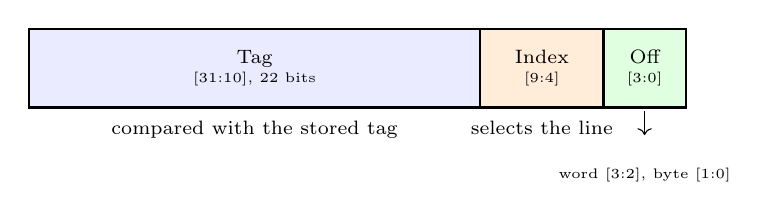
\begin{tikzpicture}[x=0.0215\columnwidth,y=1cm,font=\scriptsize]
  \draw[thick,fill=blue!8] (0,0) rectangle (22,1.0);
  \draw[thick,fill=orange!15] (22,0) rectangle (28,1.0);
  \draw[thick,fill=green!12] (28,0) rectangle (32,1.0);
  \node[align=center] at (11,0.5) {Tag\\[-1pt]\tiny [31:10], 22 bits};
  \node[align=center] at (25,0.5) {Index\\[-1pt]\tiny [9:4]};
  \node[align=center] at (30,0.5) {Off\\[-1pt]\tiny [3:0]};
  \node[below,align=center] at (11,-0.05) {compared with the stored tag};
  \node[below,align=center] at (25,-0.05) {selects the line};
  \node[below,align=center] at (30,-0.65) {\tiny word [3:2], byte [1:0]};
  \draw[->] (30,-0.05) -- (30,-0.35);
\end{tikzpicture}
\caption{Address fields: tag $[31{:}10]$, index $[9{:}4]$, offset $[3{:}0]$. Offset bits $[3{:}2]$ choose the word and $[1{:}0]$ the byte (word-aligned requests have $[1{:}0]=00$).}\label{fig:addr}
\end{figure}

\begin{figure}[t]
\centering
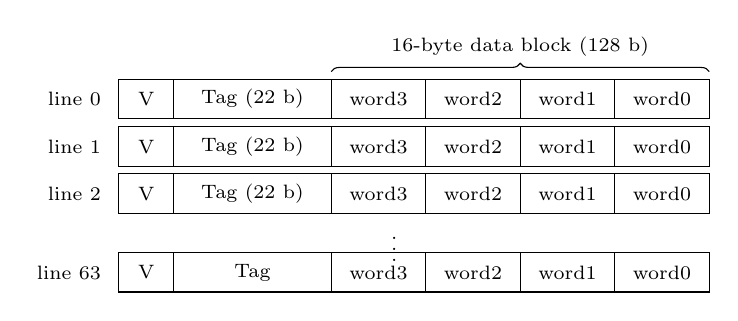
\begin{tikzpicture}[font=\scriptsize]
  \foreach \i/\y in {0/3.0,1/2.4,2/1.8} {
    \draw (0,\y) rectangle (0.7,\y+0.5); \node at (0.35,\y+0.25) {V};
    \draw (0.7,\y) rectangle (2.7,\y+0.5); \node at (1.7,\y+0.25) {Tag (22 b)};
    \foreach \w/\x in {3/2.7,2/3.9,1/5.1,0/6.3} {
      \draw (\x,\y) rectangle (\x+1.2,\y+0.5); \node at (\x+0.6,\y+0.25) {word\w};
    }
    \node[left] at (-0.1,\y+0.25) {line \i};
  }
  \node at (3.5,1.45) {$\vdots$};
  \draw (0,0.8) rectangle (0.7,1.3); \node at (0.35,1.05) {V};
  \draw (0.7,0.8) rectangle (2.7,1.3); \node at (1.7,1.05) {Tag};
  \foreach \w/\x in {3/2.7,2/3.9,1/5.1,0/6.3} {\draw (\x,0.8) rectangle (\x+1.2,1.3); \node at (\x+0.6,1.05) {word\w};}
  \node[left] at (-0.1,1.05) {line 63};
  \draw[decorate,decoration={brace,amplitude=3pt}] (2.7,3.6) -- (7.5,3.6) node[midway,above=2pt] {16-byte data block (128 b)};
\end{tikzpicture}
\caption{Cache organization: 64 lines, each with a valid bit, a 22-bit tag and a 16-byte block. Byte $i$ of a block is at bits $[8i+7{:}8i]$.}\label{fig:org}
\end{figure}

%=====================================================================
\section{Microarchitecture}\label{sec:arch}
\subsection{Overview}
Fig.~\ref{fig:block} shows the modules and their connections. The processor side uses a \code{req_valid/req_ready} request and a \code{resp_valid} response. The memory side is hidden behind a small protocol engine, so the controller never touches memory signals directly and the memory model can be replaced by any module with the same ports.

\begin{figure*}[t]
\centering
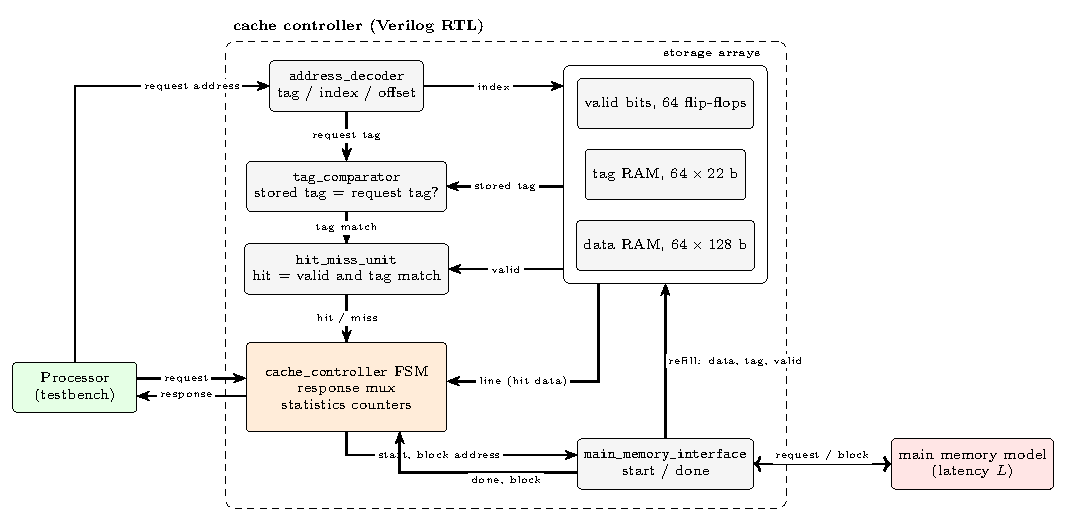
\includegraphics[width=0.92\textwidth]{block_diagram.pdf}
\caption{Block diagram of the cache controller. The address decoder drives the index to the three arrays; the FSM compares the stored tag and valid bit; refills flow from the memory interface into the arrays.}\label{fig:block}
\end{figure*}

\subsection{Modules}
\begin{table}[t]
\caption{RTL modules (\texttt{rtl/}, 354 lines in total)}\label{tab:modules}
\centering\small
\begin{tabular}{@{}p{0.40\columnwidth}p{0.52\columnwidth}@{}}
\toprule
Module & Function\\
\midrule
\code{address_decoder} & Splits the address into tag, index, offset and block address; parameter-derived widths and elaboration checks.\\
\code{cache_data_ram} & $64\times16$~B data; 16 byte-lane RAMs with synchronous read and per-byte write mask.\\
\code{cache_tag_ram} & $64\times22$~b tags; synchronous read and write.\\
\code{cache_valid_ram} & 64 flip-flops so that one reset clears every valid bit.\\
\code{main_memory_interface} & Memory protocol engine: \emph{start}/\emph{done} towards the controller; request held until memory accepts.\\
\code{cache_controller} & FSM, tag/valid comparison, response multiplexer and seven statistics counters.\\
\midrule
\multicolumn{2}{@{}l}{\emph{Simulation only (\texttt{sim/}):}}\\
\code{main_memory_model} & Behavioral memory with configurable latency and deterministic contents.\\
\code{reference_memory} & Independent golden model (32-bit words) used for checking.\\
\bottomrule
\end{tabular}
\end{table}

\subsection{Design decisions}
\begin{itemize}
\item \textbf{Synchronous-read arrays.} Data, tag and valid are read at the cycle in which a request is accepted, so the results are available in the following (LOOKUP) cycle. This models real block RAMs.
\item \textbf{Valid bits in flip-flops.} A RAM cannot be cleared in one cycle; 64 flip-flops can.
\item \textbf{Whole-block transfer.} The memory returns 128 bits at once, so a refill is one request and one response.
\item \textbf{Byte lanes.} The data RAM is built from 16 narrow RAMs. A first version that wrote a single wide array in a byte loop synthesized to about 9{,}750 flip-flops because it had 16 write ports; the byte-lane form maps to block RAM (Section~\ref{sec:synth}).
\item \textbf{Blocking cache.} One request is processed at a time.
\end{itemize}

\subsection{Hit logic}
The hit decision is a single expression; an invalid line always misses, whatever tag it holds:
\begin{lstlisting}
wire hit = rd_valid && (rd_tag == q_tag);
\end{lstlisting}
\begin{equation}
\text{hit}=V[\text{index}]\;\wedge\;\bigl(T[\text{index}]=\text{tag}_{\text{req}}\bigr).\label{eq:hit}
\end{equation}
The returned word is selected from the 128-bit line by the upper offset bits:
\begin{equation}
\text{rdata}=\text{line}\bigl[\,32\,w+31:32\,w\,\bigr],\quad w=\text{offset}[3{:}2].\label{eq:word}
\end{equation}
On a hit the line comes from the data-RAM read register. On a miss it comes from the refill block register, so a miss does not need a second RAM read.

\subsection{Interfaces}
\begin{table}[t]
\caption{Processor-side interface}\label{tab:cpuif}
\centering\small
\begin{tabular}{@{}p{0.31\columnwidth}p{0.61\columnwidth}@{}}
\toprule
Signal & Meaning\\
\midrule
\code{clk, rst_n} & Clock; active-low synchronous reset.\\
\code{req_valid, req_ready} & Request accepted on the clock edge where both are 1. \code{req_ready} is high only in IDLE.\\
\code{req_addr[31:0]} & Byte address (word aligned, below the memory size).\\
\code{resp_valid} & One-cycle pulse for every accepted request.\\
\code{resp_rdata[31:0]} & Read data, valid with \code{resp_valid}; 0 on error.\\
\code{resp_hit, resp_err} & Request was a hit / request was bad (misaligned, out of range, or a write).\\
\code{stat_*} & Seven counters (Table~\ref{tab:stats}).\\
\bottomrule
\end{tabular}
\end{table}

\emph{Memory side:} \code{mem_req_valid} is held until \code{mem_req_ready}; \code{mem_req_addr} is block aligned; \code{mem_resp_valid} is a one-cycle pulse with the 128-bit \code{mem_resp_data}. The memory model's latency parameter $L$ is the number of clock edges from request acceptance to the response pulse.

%=====================================================================
\section{Controller FSM and Timing}\label{sec:fsm}
\subsection{Flow of a request}
Fig.~\ref{fig:flow} shows the decision flow for one request. A bad request is answered at once with an error; otherwise the line is read, the tag and valid bit are checked, and the word is either returned (hit) or the block is fetched, installed and then returned (miss).

\begin{figure}[t]
\centering
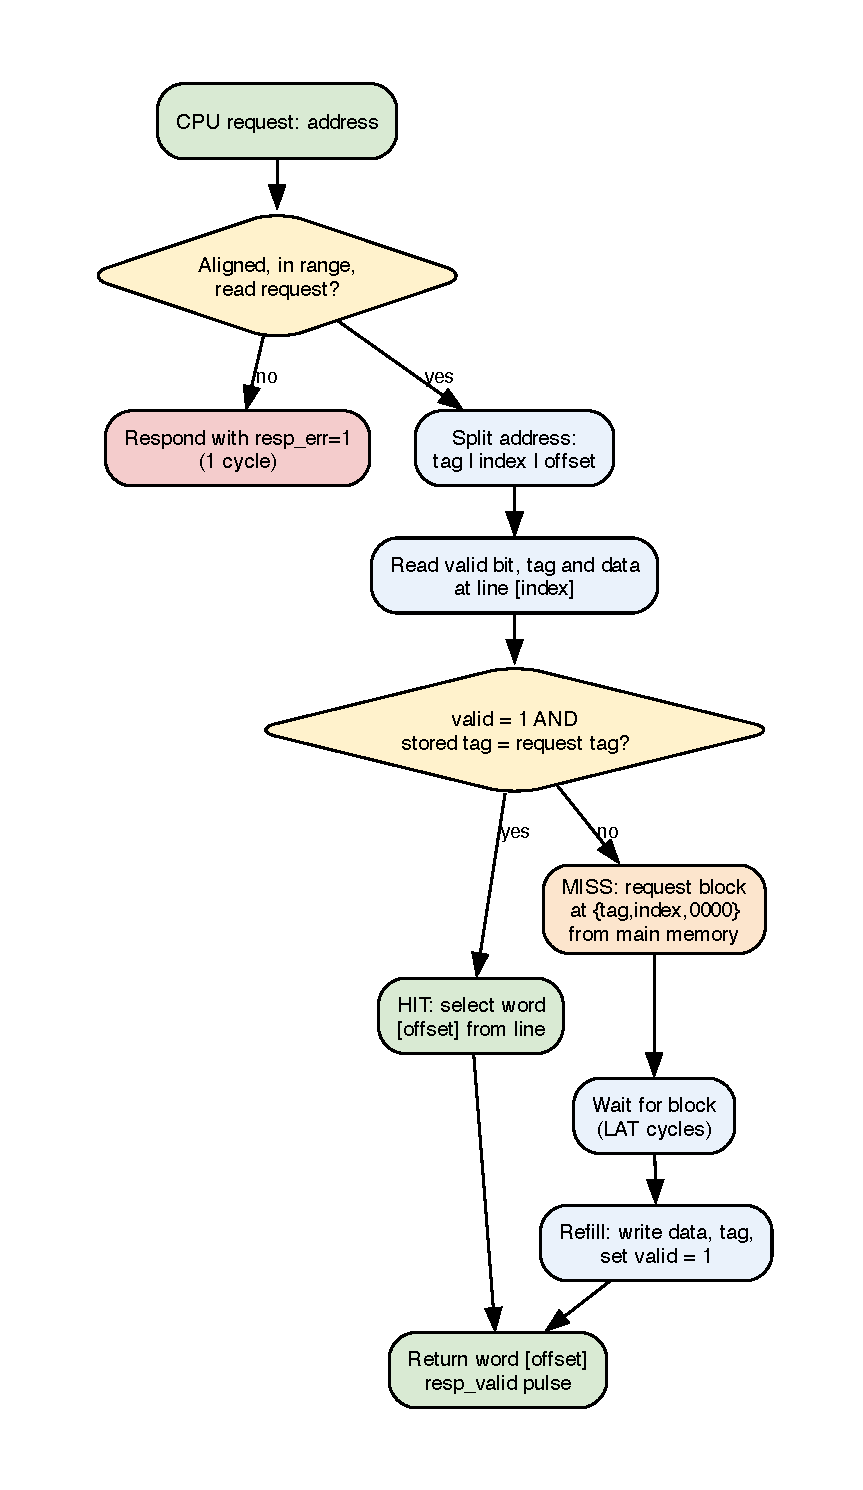
\includegraphics[width=0.78\columnwidth]{hitmiss_flow.pdf}
\caption{Request flow: lookup, hit or miss decision, refill on a miss, then response.}\label{fig:flow}
\end{figure}

\subsection{State machine}
\begin{figure*}[t]
\centering
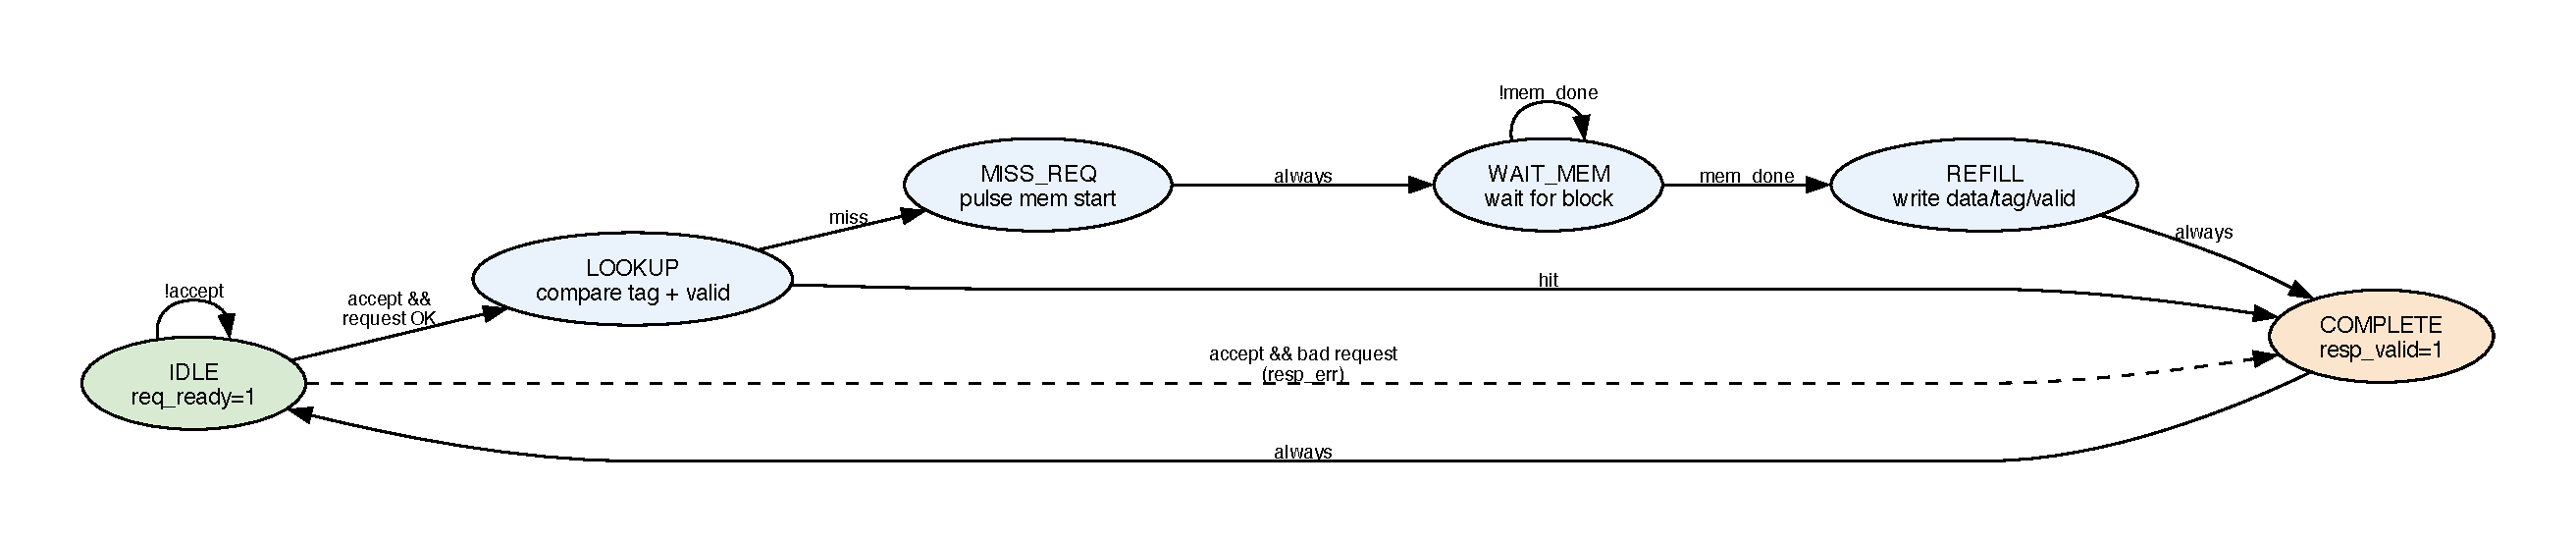
\includegraphics[width=0.95\textwidth]{fsm.pdf}
\caption{Controller FSM. Dashed behavior (bad request) goes from IDLE directly to COMPLETE; COMPLETE always returns to IDLE.}\label{fig:fsm}
\end{figure*}

\begin{table}[t]
\caption{FSM states and transitions}\label{tab:fsm}
\centering\small
\begin{tabular}{@{}p{0.2\columnwidth}p{0.4\columnwidth}p{0.28\columnwidth}@{}}
\toprule
State & Actions & Next state\\
\midrule
IDLE & \code{req_ready=1}; on accept latch address, start RAM reads & LOOKUP; COMPLETE if bad request\\
LOOKUP & RAM outputs valid; evaluate~\eqref{eq:hit}; count hit or miss & COMPLETE on hit; MISS\_REQ on miss\\
MISS\_REQ & Pulse \emph{start} with block address to the memory interface & WAIT\_MEM\\
WAIT\_MEM & Wait for the block; count wait cycles & REFILL when \emph{done}\\
REFILL & Write data, tag; set valid (all at the latched index) & COMPLETE\\
COMPLETE & \code{resp_valid=1}; return selected word & IDLE\\
\bottomrule
\end{tabular}
\end{table}

Every state has a defined next state; a default branch returns to IDLE and no latch is inferred (checked by synthesis). LOOKUP is a separate state because the RAMs read synchronously. MISS\_REQ is separate from WAIT\_MEM so exactly one start pulse is issued per miss.

\subsection{Cycle-accurate timing}
Let $E_0$ be the clock edge at which the request is accepted, and measure latency as the number of edges until \code{resp_valid} is sampled.

\emph{Hit.} $E_0$: IDLE$\to$LOOKUP. $E_1$: LOOKUP$\to$COMPLETE. \code{resp_valid} is sampled at $E_2$:
\begin{equation}
t_h=2\ \text{cycles}.\label{eq:th}
\end{equation}

\emph{Miss.} $E_0$: accept. $E_1$: LOOKUP$\to$MISS\_REQ. $E_2$: MISS\_REQ$\to$WAIT\_MEM; the memory interface captures \emph{start}. $E_3$: memory accepts the request. The memory answers $L$ edges after acceptance, the interface captures the block at $E_{4+L}$ and raises \emph{done}. $E_{5+L}$: WAIT\_MEM$\to$REFILL. $E_{6+L}$: REFILL$\to$COMPLETE. The response is sampled at $E_{7+L}$:
\begin{align}
t_m &= L+7\ \text{cycles},\label{eq:tm}\\
t_p &= t_m-t_h = L+5\ \text{cycles},\label{eq:tp}\\
\text{wait cycles per miss} &= L+4\ (\text{MISS\_REQ}+\text{WAIT\_MEM}).\label{eq:wait}
\end{align}
For $L=4$: $t_h=2$, $t_m=11$, $t_p=9$. Fig.~\ref{fig:w-cold} confirms this: the request is accepted at 30~ns and the response is sampled at 140~ns, which is 11 clock periods. These equations held for every request in every run at $L\in\{1,2,4,8,16\}$.

\subsection{Handshake rules}
A request is accepted exactly once, on the edge where \code{req_valid} and \code{req_ready} are both high. The controller latches the address at that edge, so the processor may change \code{req_addr} afterwards. A request presented while the controller is busy waits and is accepted when \code{req_ready} rises. A request withdrawn before acceptance has no effect. Exactly one \code{resp_valid} pulse follows each accepted request. These properties are checked by the testbench (Section~\ref{sec:verif}).

\subsection{Statistics counters}
\begin{table}[t]
\caption{Hardware performance counters (cleared by reset)}\label{tab:stats}
\centering\small
\begin{tabular}{@{}p{0.34\columnwidth}p{0.58\columnwidth}@{}}
\toprule
Counter & Counts\\
\midrule
\code{stat_requests} & accepted requests\\
\code{stat_hits}, \code{stat_misses} & LOOKUP outcomes (bad requests are neither)\\
\code{stat_mem_reads} & block-read transactions (one per miss)\\
\code{stat_completed} & responses delivered\\
\code{stat_cycles} & cycles since reset\\
\code{stat_mem_wait_cycles} & cycles in MISS\_REQ and WAIT\_MEM\\
\bottomrule
\end{tabular}
\end{table}

%=====================================================================
\section{Verification}\label{sec:verif}
\subsection{Strategy}
Two independent layers check every run:
\begin{enumerate}
\item A \textbf{monitor} watches the processor interface each clock. At every accepted request it computes the expected data from the reference memory and the expected hit or miss from a separate behavioral cache model written in the testbench. It checks every response and the protocol rules: one response per request, none while idle, no miss response before the memory data arrives, and no request accepted while busy.
\item \textbf{Directed checks} add explicit expectations: hit/miss pattern, latency, memory read count and alignment, and white-box checks of the valid, tag and data arrays.
\end{enumerate}
After every test the hardware counters must equal the testbench counts, memory-wait cycles must equal misses$\times(L+4)$, and the counter of memory reads must equal the reads seen on the memory bus. Each test begins with a reset. The random test uses a fixed seed, so results are reproducible. The simulator exits with a nonzero status on failure.

\subsection{Tests}
\begin{table}[t]
\caption{Directed and randomized tests (checks at $L=4$)}\label{tab:tests}
\centering\small
\begin{tabular}{@{}r p{0.52\columnwidth} r@{}}
\toprule
\# & Expected behavior & Checks\\
\midrule
1 & Cold miss: one block-aligned memory read; valid, tag, data installed & 17\\
2 & Repeated access: miss then hits; one memory read & 18\\
3 & Same-block words: one miss, three hits, no extra refill & 21\\
4 & Conflict (0 and 1024): same index, different tags; every access misses & 36\\
5 & 64 different lines: 64 misses, then 64 hits; no eviction & 399\\
6 & Sequential words: 64 misses, 192 hits; second pass all hit & 1547\\
7 & Reset: valid bits and counters clear; stale data never hits; reset mid-miss is clean & 34\\
8 & Latency: miss $=L+7$ cycles, wait $=L+4$, hit $=2$ & 18\\
9 & Handshake: held requests accepted once, in order; withdrawn requests ignored & 57\\
10 & 5000 seeded random reads vs.\ both models & 5009\\
11 & Boundary: first/last word; misaligned, out-of-range, write $\to$ error, no memory read & 43\\
\bottomrule
\end{tabular}
\end{table}

All eleven tests pass at $L=1,2,4,8,16$. Two unit tests also pass: the address decoder against plain bit slicing for 20{,}000 random addresses in two geometries, and the storage arrays (reset, tag/data read-write, read hold, byte mask).

\subsection{Does the testbench catch bugs?}
A testbench that always passes proves nothing, so thirteen faults were injected one at a time into copies of the RTL (Table~\ref{tab:mut}). The testbench must exit with failure for each.

\begin{table}[t]
\caption{Fault injection (all run with the full testbench)}\label{tab:mut}
\centering\small
\begin{tabular}{@{}p{0.6\columnwidth}p{0.3\columnwidth}@{}}
\toprule
Injected fault & Result\\
\midrule
Ignore the valid bit in the hit decision & caught\\
Ignore the tag LSB / compare only part of the tag & caught\\
Wrong word select from the line & caught\\
Refill writes data / tag / valid to the wrong line (3 faults) & caught\\
Valid bits not cleared on reset & caught\\
Miss returns stale RAM data & caught\\
Hit counter incremented on accept & caught\\
Do not wait for memory data & caught\\
Tag RAM never written & caught\\
Block address not aligned & caught\\
Ignore tag bit 21 (address bit 31) & survives\\
\bottomrule
\end{tabular}
\end{table}

The survivor is behaviorally equivalent: the memory is 64~KB, so valid addresses never have bit 31 set and that tag bit cannot change any result. An early version of the testbench missed the wrong-line refill faults because the driver kept the request address stable after acceptance; the driver now changes the address after acceptance (proving the controller uses its latched copy) and the handshake test reads its whole stream back. Fault injection of this kind follows the idea of mutation testing~\cite{demillo1978}.

%=====================================================================
\section{Waveform Analysis for Different Inputs}\label{sec:waves}
Each figure in this section was drawn from the VCD of a real Icarus Verilog run of the corresponding test. The clock period is 10~ns, the time axis starts at the beginning of the displayed window, and $L=4$ unless stated. In the figures, \code{req_addr} changes shortly after acceptance because the testbench deliberately moves the address on to show that the controller uses its latched copy.

\subsection{Cold miss}
Fig.~\ref{fig:w-cold} shows the first access to address $\mathtt{0x44}$ (index 4, tag 0), to an empty cache.
\begin{itemize}
\item At 30~ns the request is accepted and \code{req_ready} falls.
\item LOOKUP (30--40~ns): the valid bit is 0, so the access is a miss.
\item MISS\_REQ (40--50~ns): \code{mem_req_valid} rises at 50~ns for one request.
\item WAIT\_MEM (50--120~ns, $L+3=7$ cycles): memory responds; \code{mem_resp_valid} is the pulse at 100--110~ns.
\item REFILL (120--130~ns): the block is written; COMPLETE (130--140~ns): \code{resp_valid} with the word $\mathtt{0xab045db6}$ (word 1 of the block based at $\mathtt{0x40}$); \code{resp_hit}=0.
\end{itemize}
The total from acceptance to sampled response is 110~ns, or 11 cycles, matching~\eqref{eq:tm}.

\begin{figure*}[t]
\centering
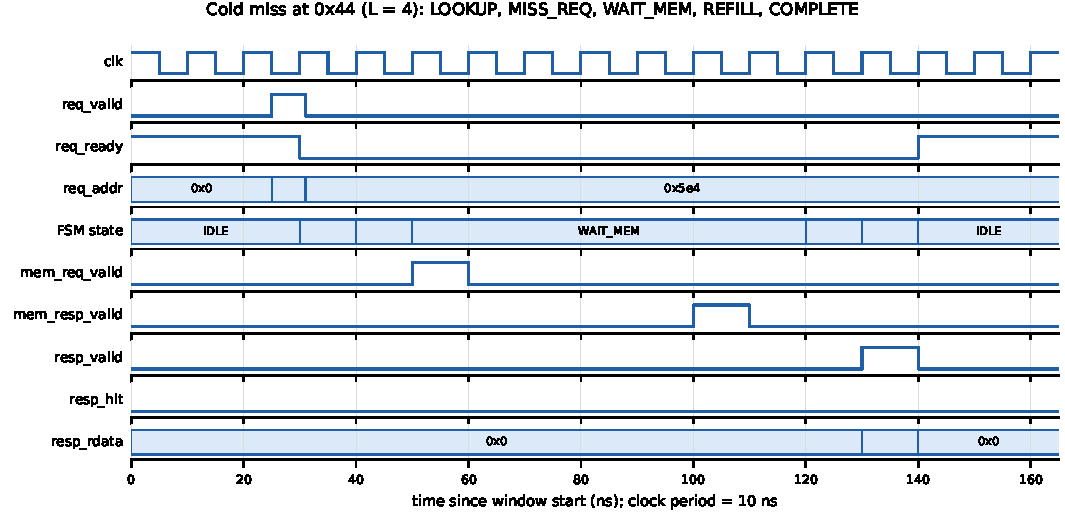
\includegraphics[width=\textwidth]{wave_cold_miss.pdf}
\caption{Cold miss at $\mathtt{0x44}$, $L=4$: five FSM states, one memory request, 11 cycles from accept to response.}\label{fig:w-cold}
\end{figure*}

\subsection{Repeated access}
Fig.~\ref{fig:w-rep} accesses $\mathtt{0x80}$ three times. The first access is a miss and takes 11 cycles; the next two find a valid line with a matching tag, so the FSM goes IDLE$\to$LOOKUP$\to$COMPLETE, \code{resp_hit} is 1, no memory request is made and each takes 2 cycles. This is \emph{temporal locality} in action.

\begin{figure*}[t]
\centering
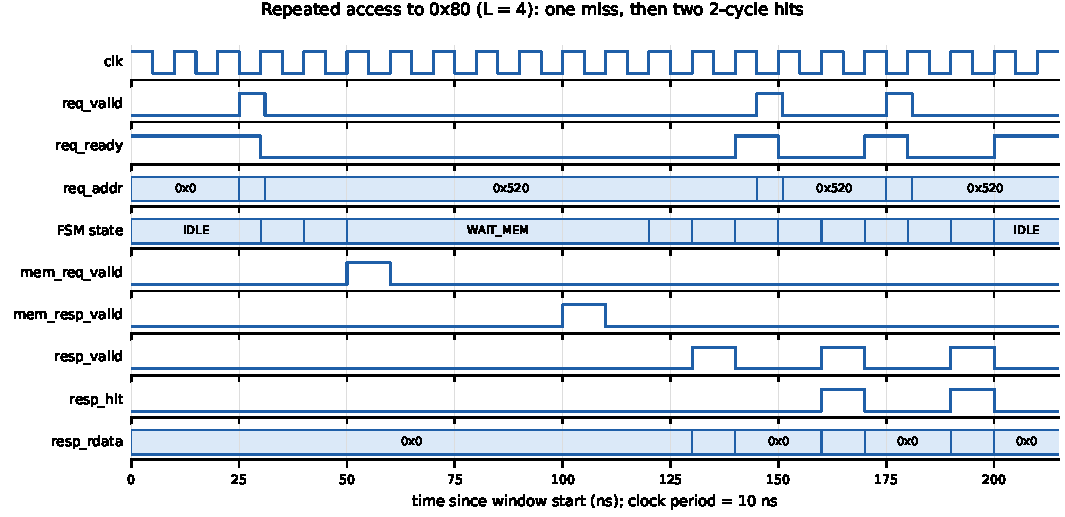
\includegraphics[width=\textwidth]{wave_repeated.pdf}
\caption{Repeated access: one miss followed by two 2-cycle hits with no memory activity.}\label{fig:w-rep}
\end{figure*}

\subsection{Same-block accesses}
Fig.~\ref{fig:w-same} reads four different words of one block ($\mathtt{0x108}$, $\mathtt{0x100}$, $\mathtt{0x104}$, $\mathtt{0x10C}$). Only the first causes a refill; the others hit because the whole 16-byte block arrived together. This is \emph{spatial locality}, and it also shows that the controller does not refill a block it already holds.

\begin{figure*}[t]
\centering
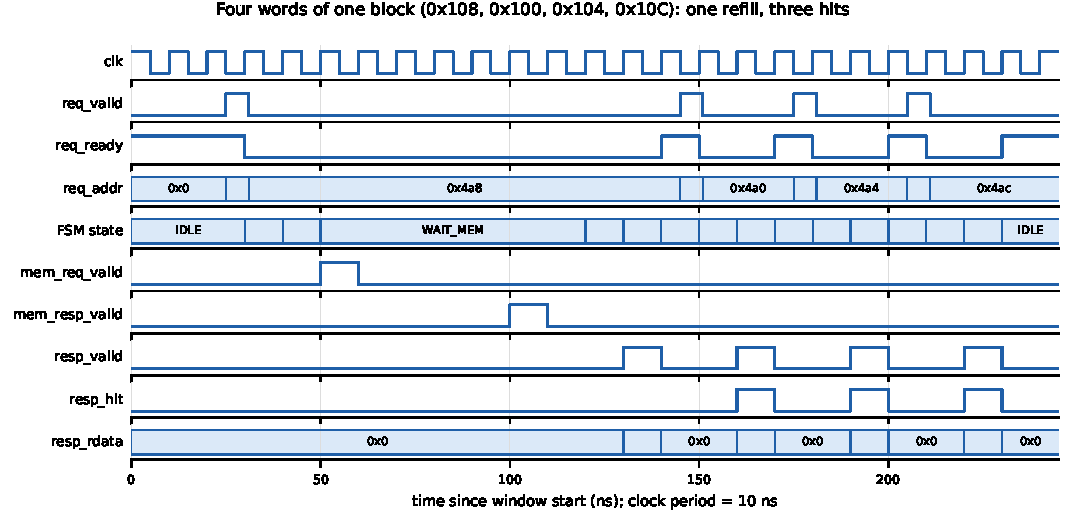
\includegraphics[width=\textwidth]{wave_same_block.pdf}
\caption{Four words of one block: one refill, three hits.}\label{fig:w-same}
\end{figure*}

\subsection{Direct-mapped conflict}
Addresses $\mathtt{0x0}$ and $\mathtt{0x400}$ share index 0 but have tags 0 and 1. Fig.~\ref{fig:w-conf} alternates between them. Every access finds a valid line whose tag does not match, so every access is a miss and every \code{mem_req_addr} alternates between $\mathtt{0x0}$ and $\mathtt{0x400}$; \code{resp_hit} never rises. Yet 63 of the 64 lines are unused: this is a pure conflict miss. A 2-way cache would hold both blocks.

\begin{figure*}[t]
\centering
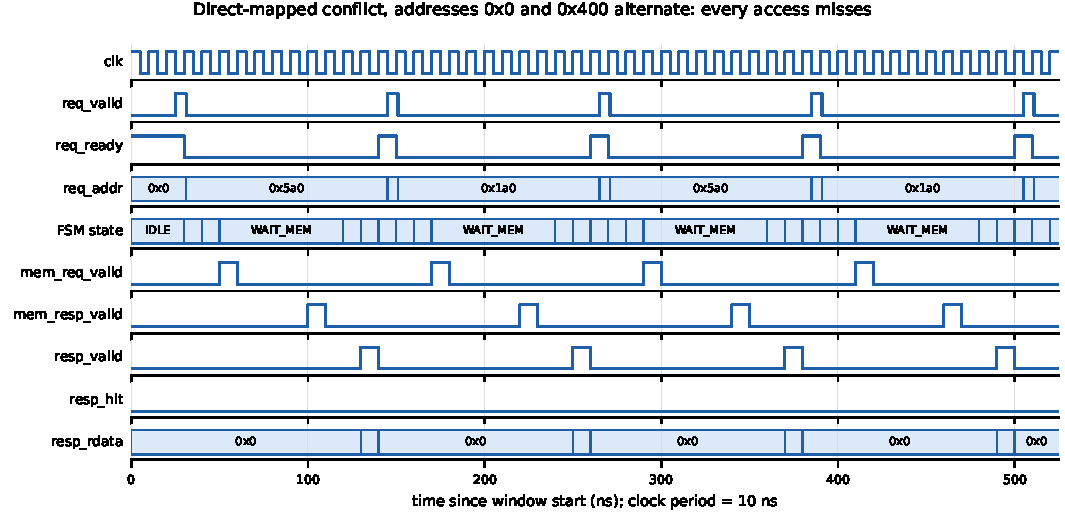
\includegraphics[width=\textwidth]{wave_conflict.pdf}
\caption{Conflict: addresses 0 and 1024 evict each other; every access is a miss and causes a block read.}\label{fig:w-conf}
\end{figure*}

\subsection{Sequential access}
Fig.~\ref{fig:w-seq} shows the first six sequential words. Words 0 to 3 lie in block 0: one miss and three hits. Word 4 starts block 1 and misses again. With 4 words per block, the steady-state miss rate for word-sequential access is $4/B=0.25$.

\begin{figure*}[t]
\centering
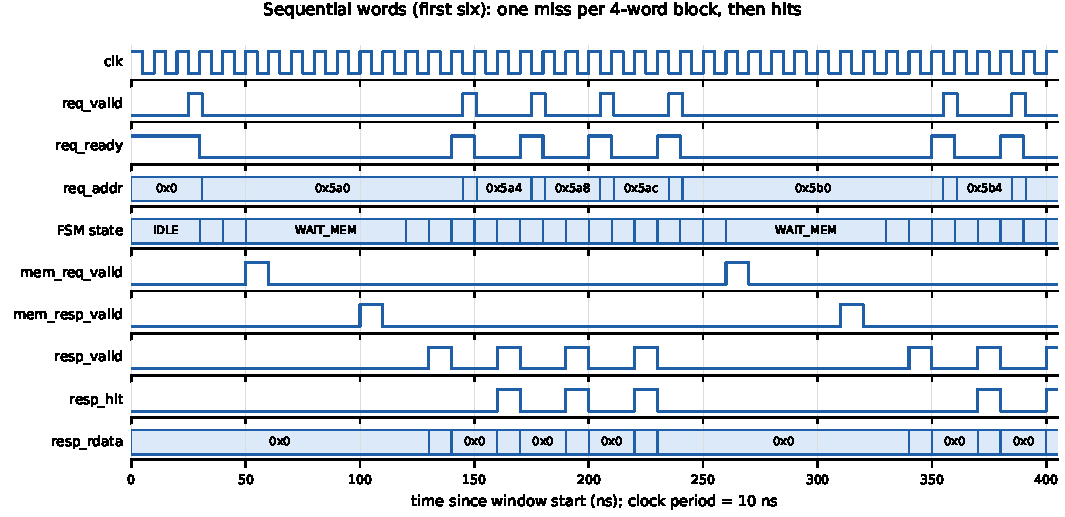
\includegraphics[width=\textwidth]{wave_sequential.pdf}
\caption{Sequential words: one miss per four-word block, then hits.}\label{fig:w-seq}
\end{figure*}

\subsection{Effect of memory latency}
Fig.~\ref{fig:w-lat} runs the same cold miss with $L=1$ and $L=16$. Only WAIT\_MEM changes: it is 4 cycles long at $L=1$ and 19 cycles at $L=16$ ($L+3$), giving 8 and 23 total cycles ($L+7$). LOOKUP, MISS\_REQ, REFILL and COMPLETE keep their one-cycle length, and the controller always waits for \code{mem_resp_valid} before responding.

\begin{figure*}[t]
\centering
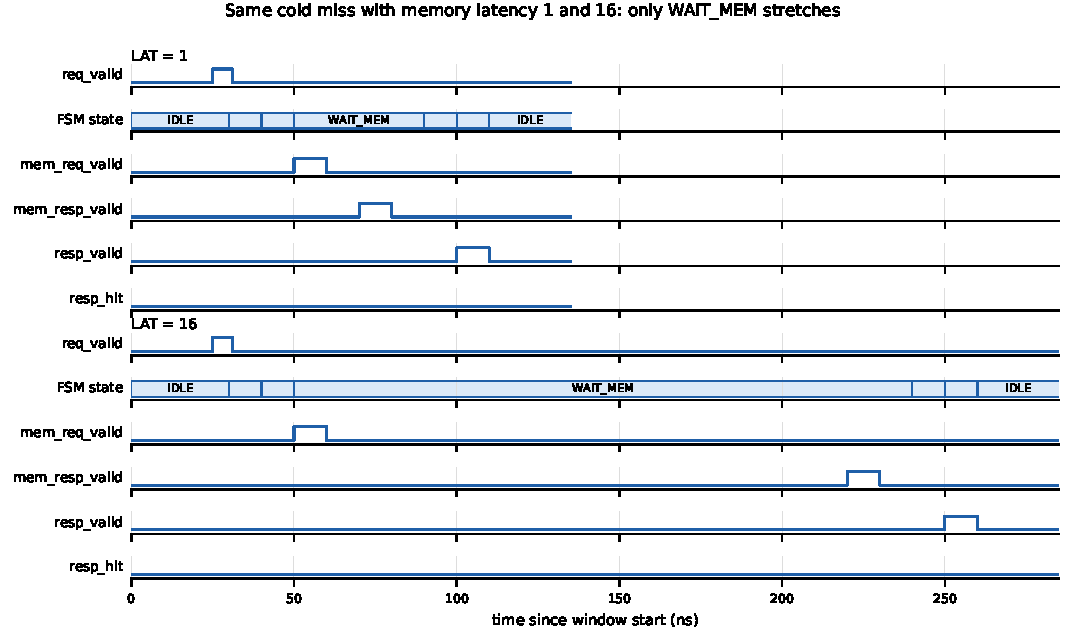
\includegraphics[width=\textwidth]{wave_latency.pdf}
\caption{The same miss with $L=1$ (top) and $L=16$ (bottom): the FSM waits in WAIT\_MEM until memory answers.}\label{fig:w-lat}
\end{figure*}

\subsection{Request handshake under load}
In Fig.~\ref{fig:w-hand} the processor keeps \code{req_valid} high and presents the next address while the controller is busy. \code{req_ready} is high for one cycle (the IDLE cycle) per request, and one request is accepted per ready pulse: five requests, five \code{resp_valid} pulses, none lost, none duplicated, in order. The requests include both misses and a hit, showing that handshake behavior does not depend on the outcome.

\begin{figure*}[t]
\centering
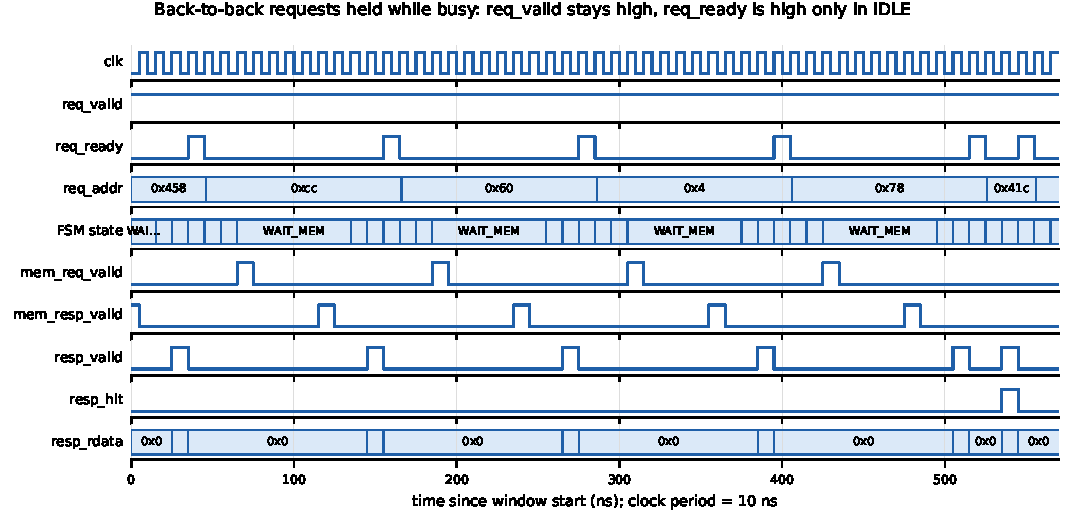
\includegraphics[width=\textwidth]{wave_handshake.pdf}
\caption{Continuous requests: acceptance only on \code{req_ready}, one response per request.}\label{fig:w-hand}
\end{figure*}

\subsection{Reset during a miss}
Fig.~\ref{fig:w-rst} shows an abort. A request is accepted and the controller requests the block (\code{mem_req_valid} at 125~ns). At 130~ns \code{rst_n} falls. The FSM and the memory interface return to idle, the memory never delivers the block to the cache (no \code{mem_resp_valid} follows) and no \code{resp_valid} appears. The testbench then confirms that the valid bit for that line is still 0 and that the next access to the same address is a clean miss.

\begin{figure*}[t]
\centering
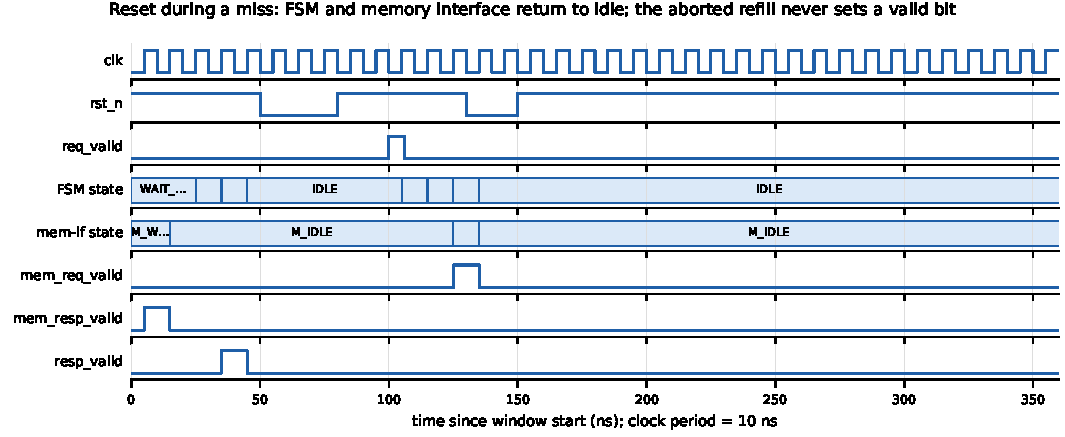
\includegraphics[width=\textwidth]{wave_reset.pdf}
\caption{Reset in the middle of a miss: clean return to idle, no stray response, no valid bit set.}\label{fig:w-rst}
\end{figure*}

\subsection{Boundary and error requests}
Fig.~\ref{fig:w-bnd} shows requests that must be rejected: misaligned addresses (1, 2, 3), the first address past the 64~KB memory ($\mathtt{0x10000}$), $\mathtt{0xFFFFFFFC}$, and a write request. Each is answered in one cycle with \code{resp_err}=1 and data 0, \code{mem_req_valid} never rises, and none of them counts as a hit or a miss.

\begin{figure*}[t]
\centering
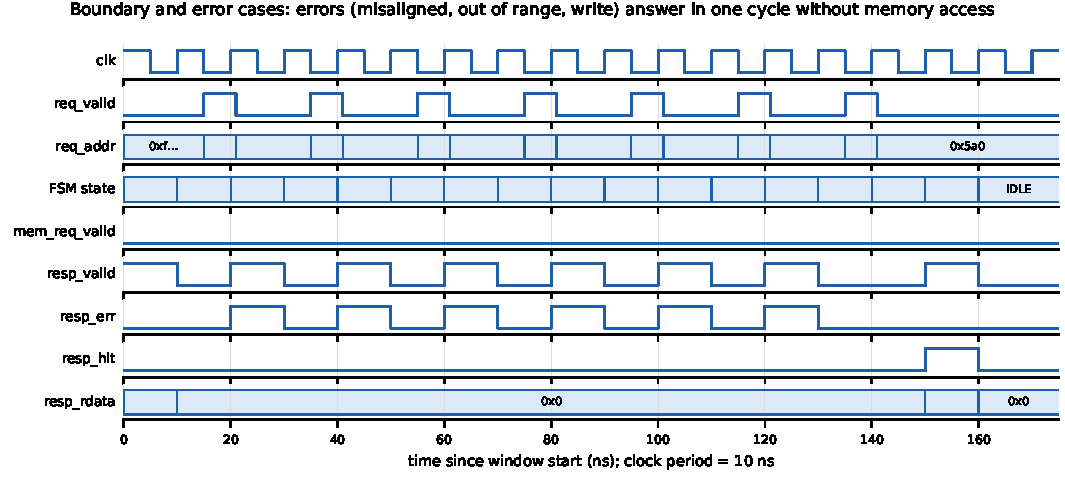
\includegraphics[width=\textwidth]{wave_boundary.pdf}
\caption{Error responses: one cycle, \code{resp_err}=1, no memory access.}\label{fig:w-bnd}
\end{figure*}

\subsection{Randomized input}
Fig.~\ref{fig:w-rand} is a slice of the seeded random test: addresses are scattered, hits and misses interleave, and idle gaps appear between requests. Every one of the 5000 responses in the full test is compared with the models.

\begin{figure*}[t]
\centering
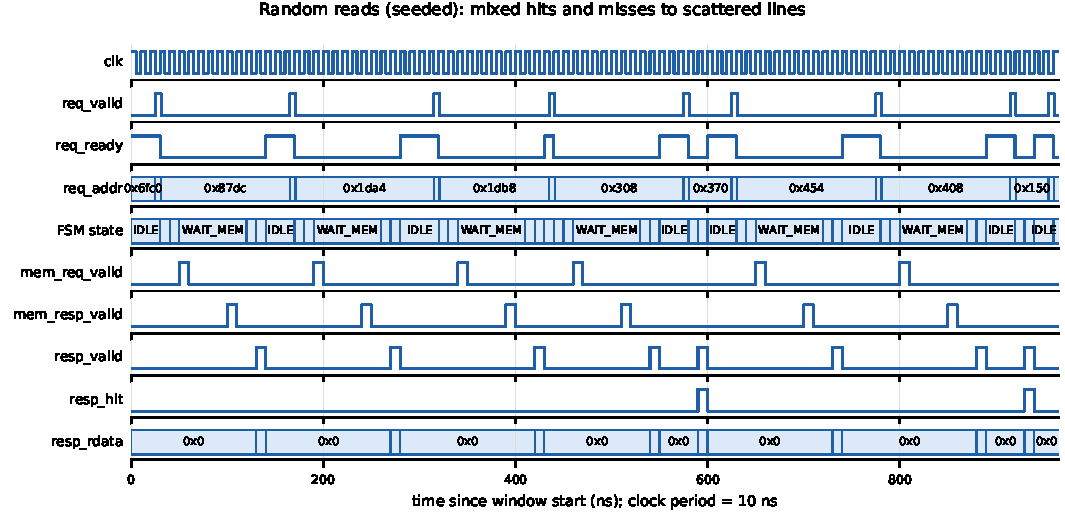
\includegraphics[width=\textwidth]{wave_random.pdf}
\caption{Random reads: hits and misses in arbitrary order, with idle gaps.}\label{fig:w-rand}
\end{figure*}

%=====================================================================
\section{Performance Analysis}\label{sec:perf}
\subsection{Method}
Five address traces were replayed with back-to-back requests from a cold cache, at $L\in\{1,4,8,16\}$. For every request, the testbench measured the accept-to-response latency and classified it as a hit or a miss using the controller's \code{resp_hit}; the controller's own counters were required to agree. A Python script computed the metrics from the printed counters. Table~\ref{tab:workloads} describes the workloads.

\begin{table}[t]
\caption{Workloads}\label{tab:workloads}
\centering\small
\begin{tabular}{@{}p{0.2\columnwidth}p{0.72\columnwidth}@{}}
\toprule
Name & Description\\
\midrule
repeated & 2000 reads cycling over 16 hot words (4 blocks)\\
sequential & one pass over 16~KB, 4096 words\\
random & 4000 uniform random words over the whole 64~KB\\
conflict & 2000 reads alternating between addresses 0..12 and 1024..1036\\
random\_hot & 4000 reads: 80\% in a 512-byte hot region, 20\% anywhere\\
\bottomrule
\end{tabular}
\end{table}

\subsection{Results}
\begin{table}[t]
\caption{Results at memory latency $L=4$ (measured)}\label{tab:perf}
\centering\small
\begin{tabular}{@{}lrrrrrr@{}}
\toprule
Workload & Req. & Hits & Misses & Hit \% & Miss \% & AMAT\\
\midrule
repeated & 2000 & 1996 & 4 & 99.8 & 0.2 & 2.02\\
sequential & 4096 & 3072 & 1024 & 75.0 & 25.0 & 4.25\\
random & 4000 & 55 & 3945 & 1.4 & 98.6 & 10.88\\
conflict & 2000 & 0 & 2000 & 0.0 & 100.0 & 11.00\\
random\_hot & 4000 & 2805 & 1195 & 70.1 & 29.9 & 4.69\\
\bottomrule
\end{tabular}
\end{table}

\begin{table}[t]
\caption{AMAT in cycles versus memory latency (measured)}\label{tab:amat}
\centering\small
\begin{tabular}{@{}lrrrr@{}}
\toprule
Workload & $L=1$ & $L=4$ & $L=8$ & $L=16$\\
\midrule
repeated & 2.01 & 2.02 & 2.03 & 2.04\\
sequential & 3.50 & 4.25 & 5.25 & 7.25\\
random & 7.92 & 10.88 & 14.82 & 22.71\\
conflict & 8.00 & 11.00 & 15.00 & 23.00\\
random\_hot & 3.79 & 4.69 & 5.88 & 8.27\\
\bottomrule
\end{tabular}
\end{table}

\begin{figure}[t]
\centering
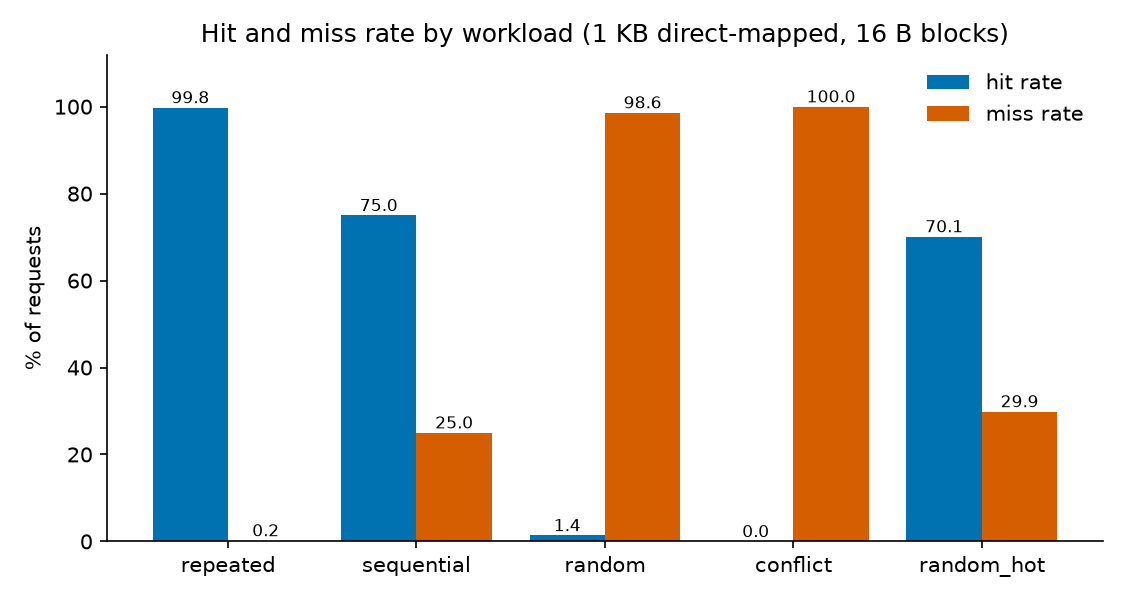
\includegraphics[width=\columnwidth]{hit_miss_rate.png}
\caption{Hit and miss rates by workload (1~KB direct-mapped, 16-byte blocks, $L=4$).}\label{fig:hm}
\end{figure}

\begin{figure}[t]
\centering
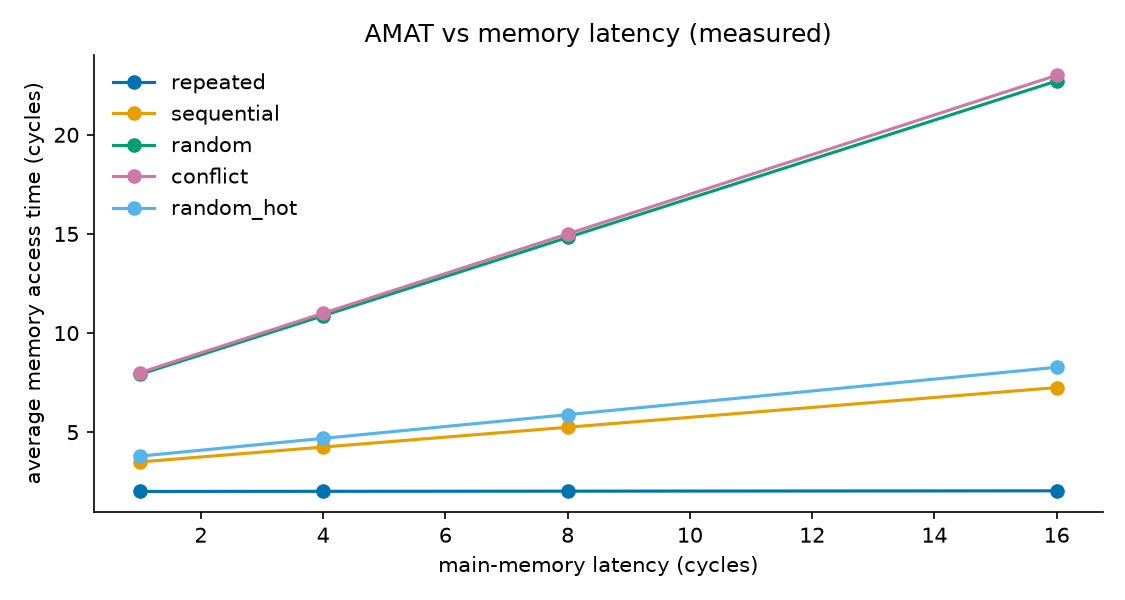
\includegraphics[width=\columnwidth]{amat_vs_latency.png}
\caption{Measured AMAT versus memory latency; the slope of each line is its miss rate.}\label{fig:amat}
\end{figure}

\subsection{AMAT verification}
With $t_h=2$ and $t_p=L+5$, equation~\eqref{eq:amat} becomes $\text{AMAT}=2+m\,(L+5)$. For \emph{sequential} at $L=4$: $2+0.25\times 9=4.25$, equal to the measured average latency. The script compares the formula with the directly measured average latency for all 20 runs, and they agree to within $10^{-9}$ in every run. Differentiating, $\partial\,\text{AMAT}/\partial L=m$: for sequential the AMAT rises from 3.50 to 4.25 to 5.25 to 7.25 as $L$ goes 1, 4, 8, 16, i.e.\ 0.25 per cycle, and for conflict ($m=1$) 1.00 per cycle, as Fig.~\ref{fig:amat} shows. The throughput figure (cycles per request) is about one cycle higher than AMAT because the controller spends one IDLE cycle before accepting the next request; this is not part of AMAT.

\subsection{Analytical checks against theory}
\begin{itemize}
\item \textbf{repeated:} only compulsory misses, one for each of the 4 distinct blocks: $m=4/2000=0.2\%$, exactly as measured.
\item \textbf{sequential:} $4096$ words $/\,4$ words per block $=1024$ misses, $m=25\%$, exactly as measured.
\item \textbf{conflict:} two blocks in one line $\Rightarrow$ $m=100\%$, as measured.
\item \textbf{random:} for uniformly random addresses, an access hits if its line holds the same block, which has probability about $C/M=1\text{~KB}/64\text{~KB}=1/64\approx1.6\%$. Measured: 1.4\% (cold-start misses lower it slightly).
\item \textbf{random\_hot:} let a fraction $p=0.8$ of accesses go to $H=32$ hot blocks (each in its own line) and $1-p$ go uniformly to $N=64$ lines. For one hot line, hot accesses arrive at rate $\lambda_h=p/H=0.025$ per request, and a wide access evicts it at rate $\lambda_e=(1-p)/N=0.0031$. The chance that the next event is a hot access (a hit) is $\lambda_h/(\lambda_h+\lambda_e)=0.889$, so $h\approx p\cdot0.889=0.711$ (wide accesses almost never hit). Measured: 0.701; the remaining difference is the 32 compulsory misses ($32/4000=0.8\%$).
\end{itemize}
The agreement between these simple models and the simulation supports the controller's correctness and the measurement method.

%=====================================================================
\section{Synthesis Estimates}\label{sec:synth}
The RTL was synthesized with Yosys using a technology-independent flow and an FPGA-style flow that maps to iCE40 primitives. The iCE40 library is used only as a representative resource model. \emph{These are software estimates: the design was not placed, routed or run on hardware, and no clock frequency is claimed.}

\begin{table}[t]
\caption{Yosys estimates for \code{cache_controller}}\label{tab:synth}
\centering\small
\begin{tabular}{@{}lr@{}}
\toprule
\multicolumn{2}{@{}l}{\emph{FPGA-style mapping (iCE40 cells, flat)}}\\
LUT4 & 635\\
Carry cells & 230\\
Flip-flops & 487\\
4~Kbit block RAMs & 18\\
\midrule
\multicolumn{2}{@{}l}{\emph{Technology-independent gates (flat)}}\\
Total cells & 26{,}160\\
Flip-flops & 10{,}237\\
\bottomrule
\end{tabular}
\end{table}

\emph{Memory inference.} All 17 arrays (16 data byte lanes and the tag array, which needs two blocks for its 22-bit width) map to block RAM. Without RAM blocks, the arrays become about 9{,}600 flip-flops plus multiplexers (the 10{,}237 flip-flops above), which explains why RAM inference matters. The first coding style of the data RAM, a single wide array with a per-byte write loop, had 16 write ports and could not be mapped; restructuring it into byte lanes fixed this, and the whole test suite was re-run afterwards and passes.

\emph{Observations.} (i) Block RAM is under-used: 18 blocks provide 73{,}728 bits for about 9{,}600 stored bits, because each $64\times8$ lane occupies a whole block. (ii) Of the 487 flip-flops, the seven 32-bit statistics counters account for 224, and they use 225 of the 230 carry cells; a production design would make them optional. The rest are the refill block and address registers (160), the valid bits (65), the latched request address (32) and a few state bits. (iii) The RTL produces no warnings and infers no latches. No timing analysis was done: it would need place-and-route, a target device and constraints.

%=====================================================================
\section{Interactive Waveform Portal}\label{sec:portal}
\subsection{Purpose}
GTKWave is the standard viewer for VCD files, but a typical workflow requires several manual steps. The portal adds a one-click path: choose a test scenario, run the real simulation, and inspect the waveform next to an FSM diagram and the cache contents. The original VCD is always kept and can be downloaded for GTKWave.

\subsection{Architecture}
\begin{figure*}[t]
\centering
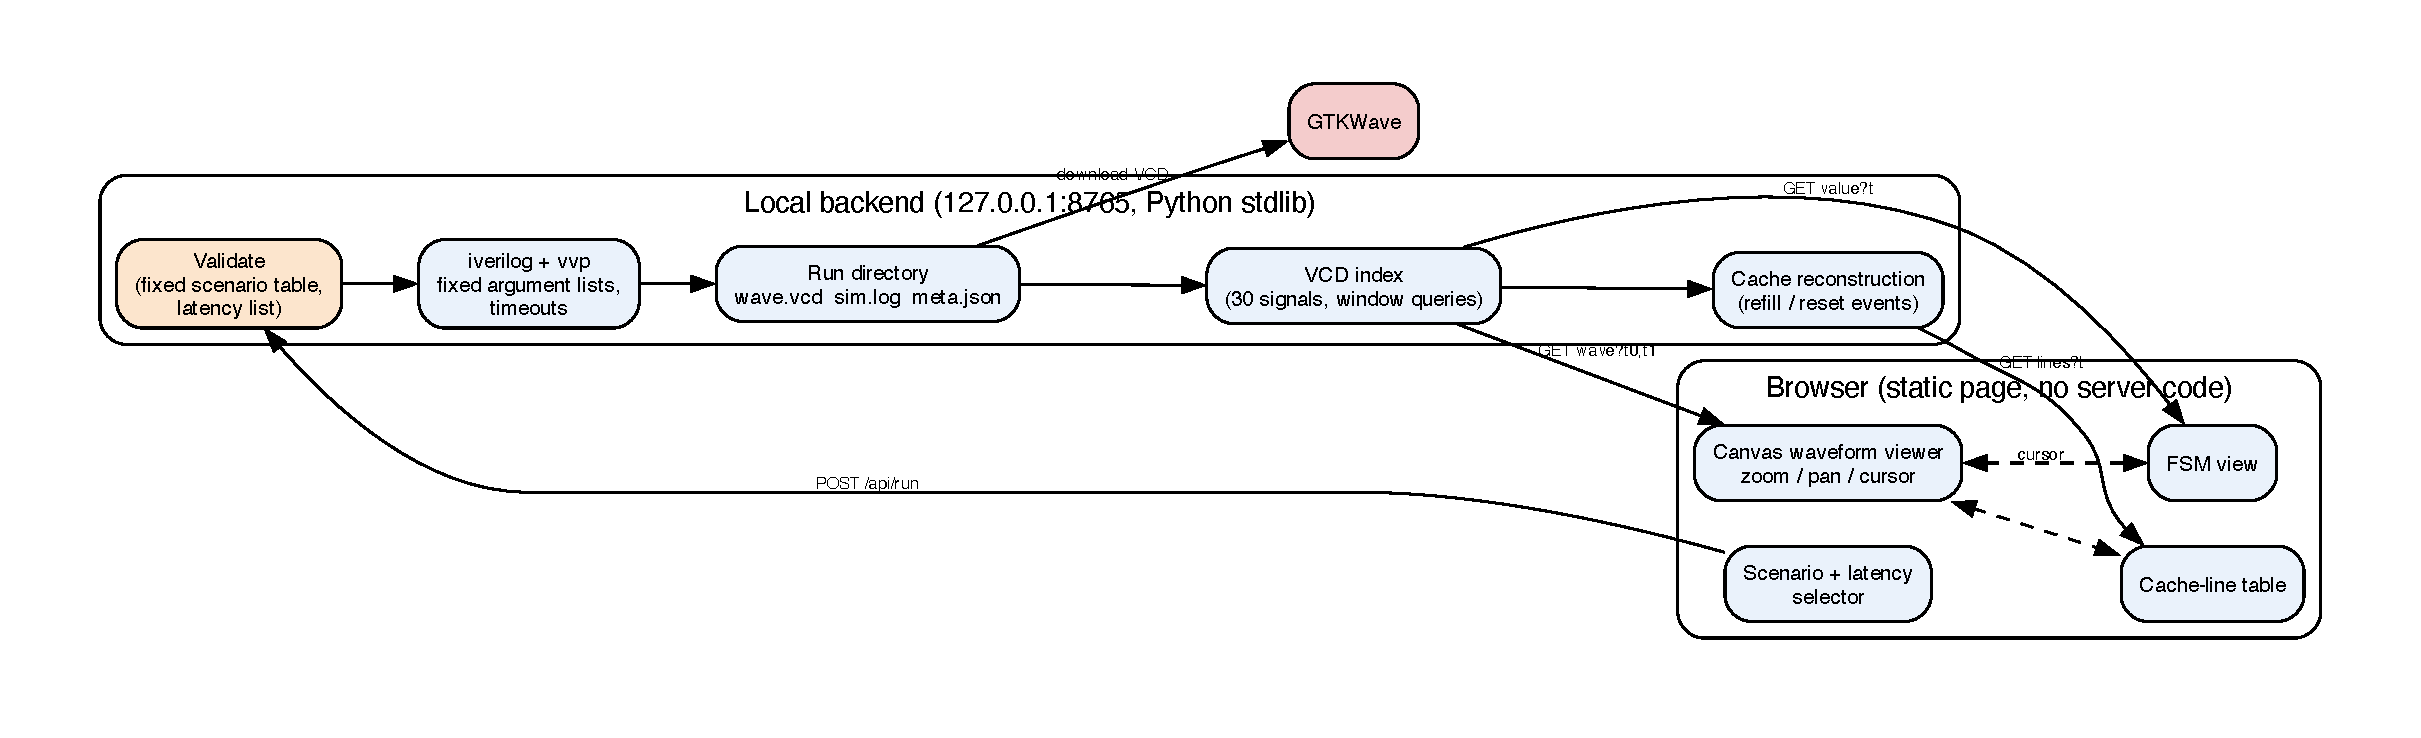
\includegraphics[width=0.95\textwidth]{portal_arch.pdf}
\caption{Portal architecture: the browser only displays data; simulations run on a local backend with fixed commands.}\label{fig:parch}
\end{figure*}

Fig.~\ref{fig:parch} shows the design. The backend is a Python standard-library server bound to \code{127.0.0.1}. When the user presses \emph{Compile \& run}, the browser sends only a scenario name and a latency. The backend checks them against a fixed table (11 tests, the full suite, and a 5000-request random run; latencies 1, 2, 4, 8, 16), then runs \code{iverilog} and \code{vvp} with fixed argument lists, no shell and timeouts. The testbench writes \code{wave.vcd} with \texttt{\$dumpfile} and \texttt{\$dumpvars}. The run directory (VCD, log, metadata) is kept, and a VCD index serves the browser through small window queries.

\subsection{Features}
\begin{itemize}
\item \textbf{Results panel:} compiler messages, each test's expected and actual line, PASS/FAIL, the exact commands run, and the raw log.
\item \textbf{Run provenance banner:} run identifier, scenario, latency, time, design hash, VCD path, size and SHA-256.
\item \textbf{Waveform:} 30 signals in collapsible groups (clock and reset, CPU request, CPU response, cache controller, memory interface, statistics, testbench); zoom (wheel or buttons), horizontal navigation (drag, slider, shift-wheel), a movable time cursor (click, ruler drag, arrow keys), signal selection, and bus values in hex, binary or decimal. States are shown by name (IDLE, LOOKUP, \ldots) and unknown values are marked in red.
\item \textbf{Synchronized views:} the FSM diagram highlights the state at the cursor and shows the latched address split into tag, index and offset together with the counters; the cache-line table shows each line's valid bit, tag and data at the cursor.
\item \textbf{Download VCD} and a copyable GTKWave command.
\end{itemize}

\begin{figure*}[t]
\centering
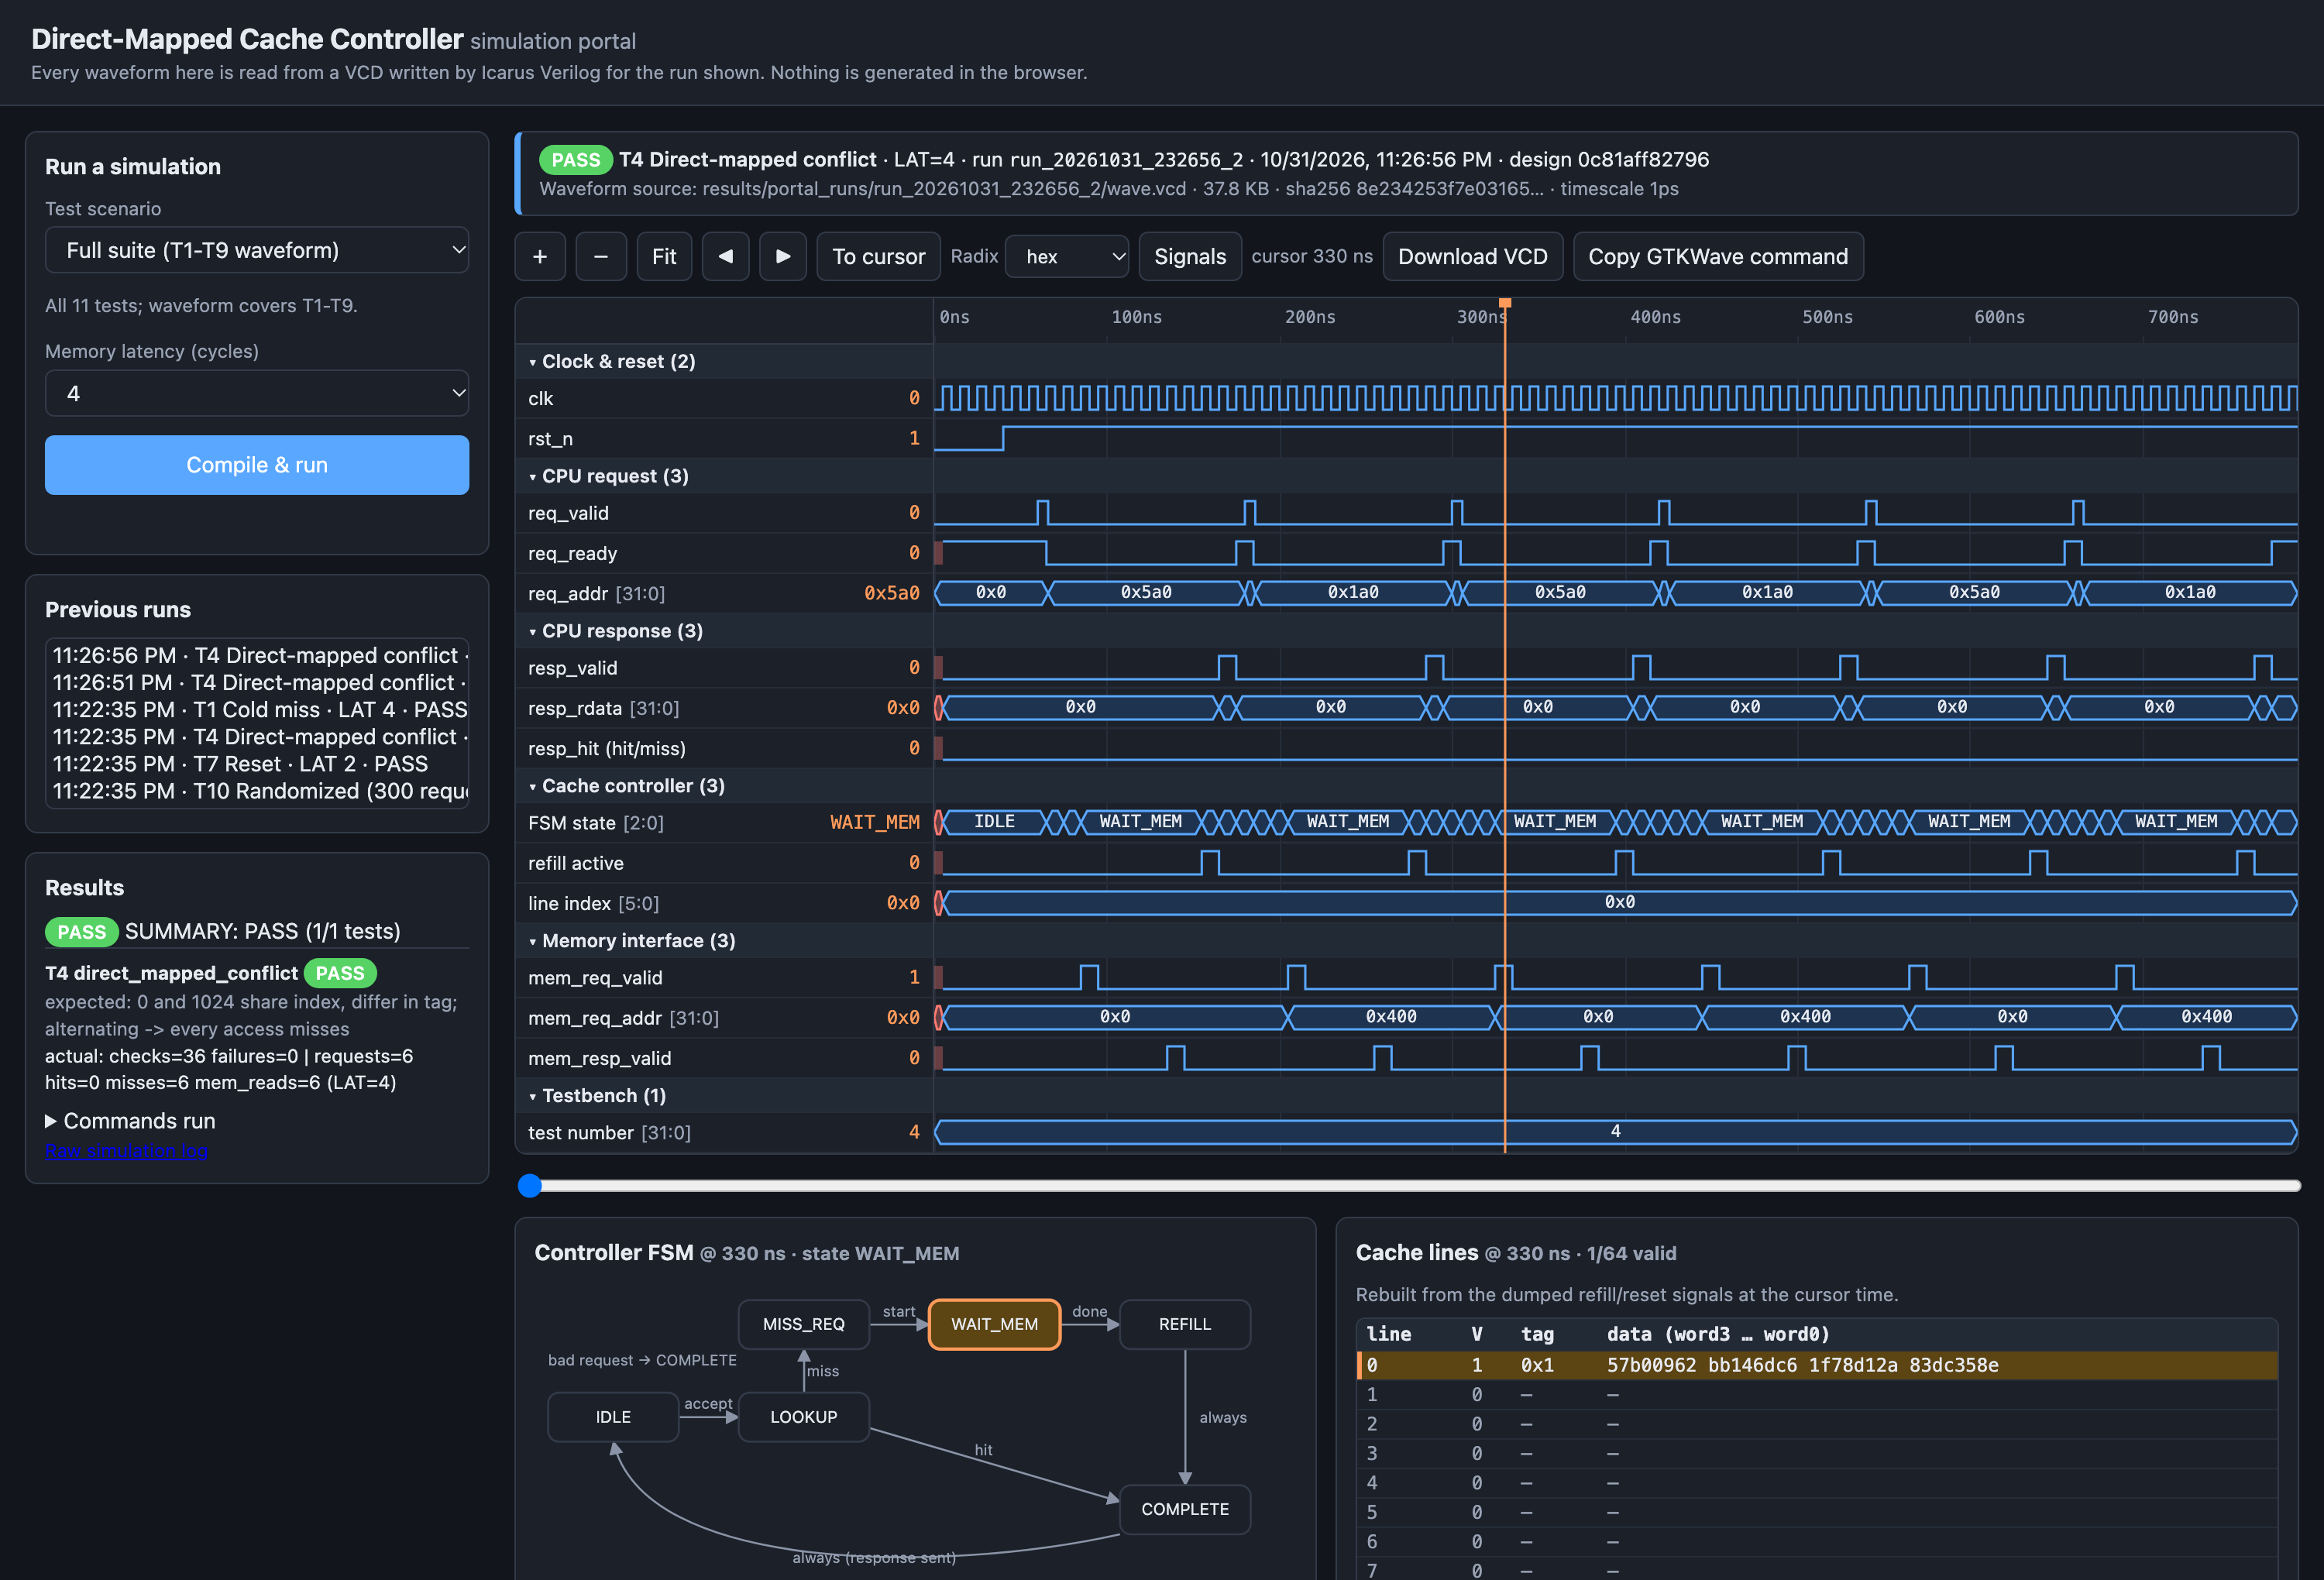
\includegraphics[width=0.96\textwidth]{portal_overview.png}
\caption{Portal: run controls, results and run banner (left, top), waveform with cursor at 330~ns during a conflict test (center), FSM highlighting WAIT\_MEM and the cache-line table (bottom).}\label{fig:p-over}
\end{figure*}

\begin{figure*}[t]
\centering
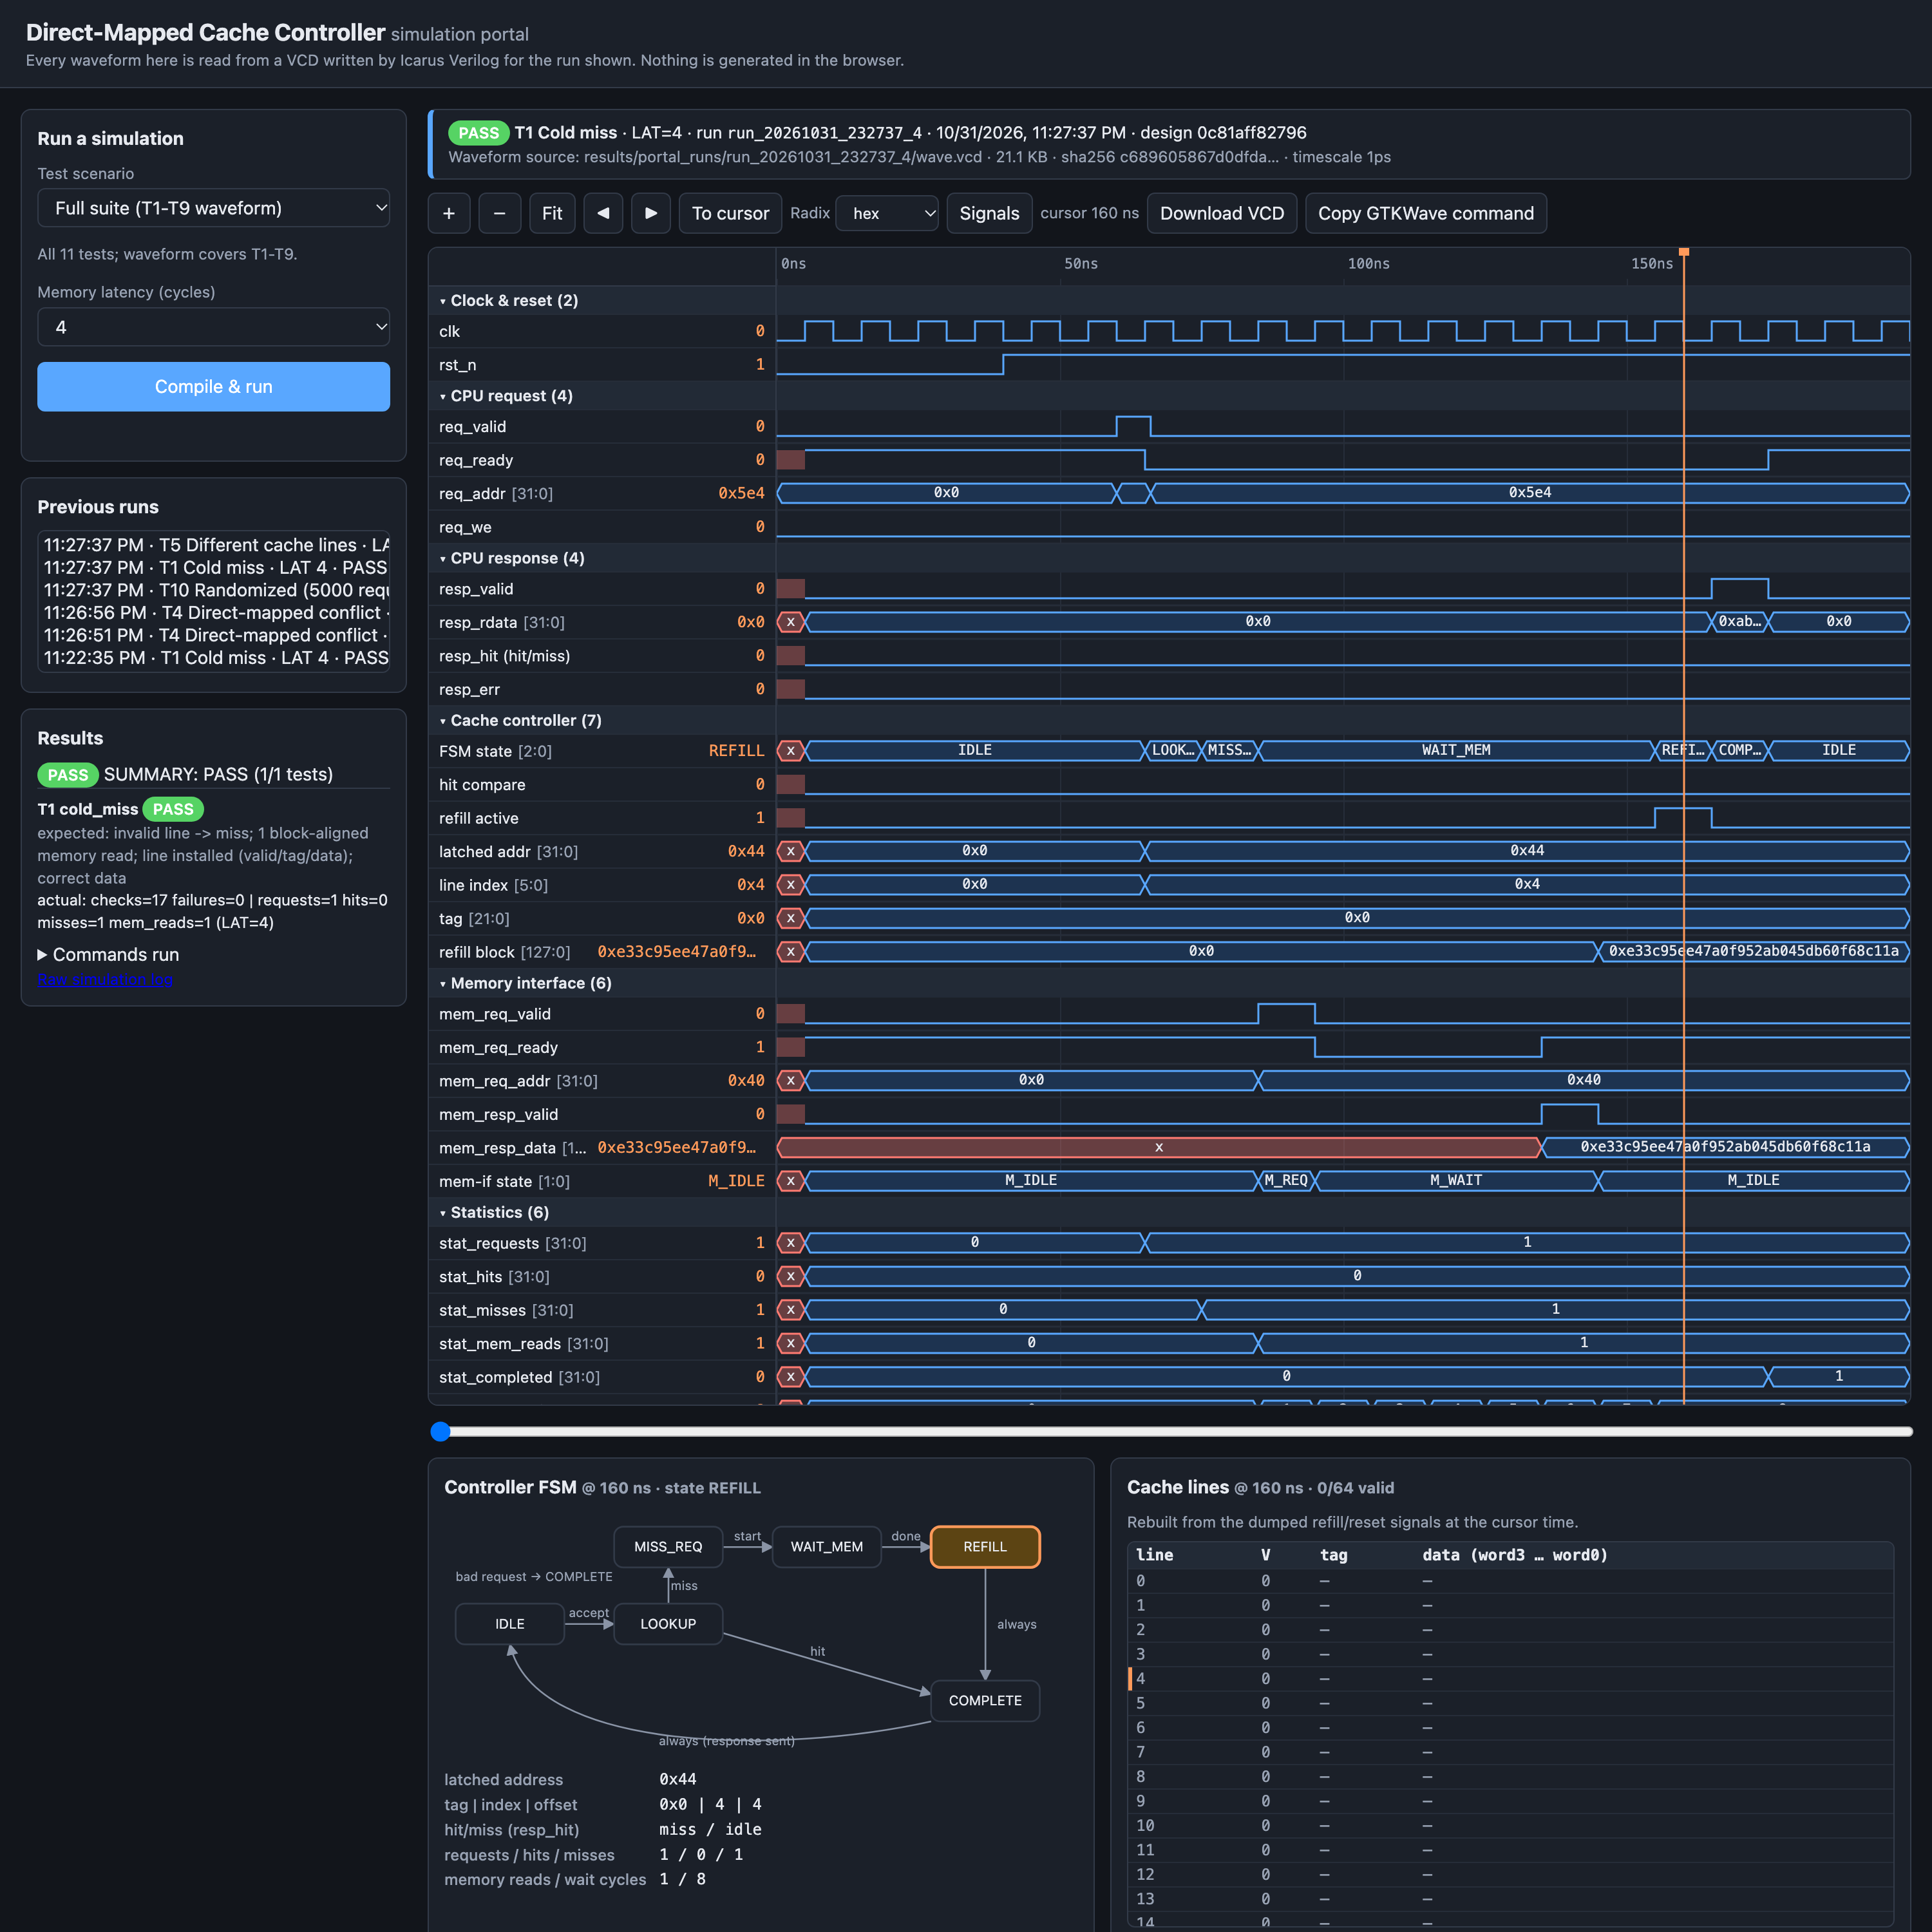
\includegraphics[width=0.66\textwidth]{portal_zoom_miss.png}
\caption{Cold miss at 160~ns with every signal shown. The FSM view highlights REFILL, \code{refill block} carries the data from memory, and the cache table is still empty at this instant because the write lands on the next clock edge.}\label{fig:p-zoom}
\end{figure*}

\begin{figure*}[t]
\centering
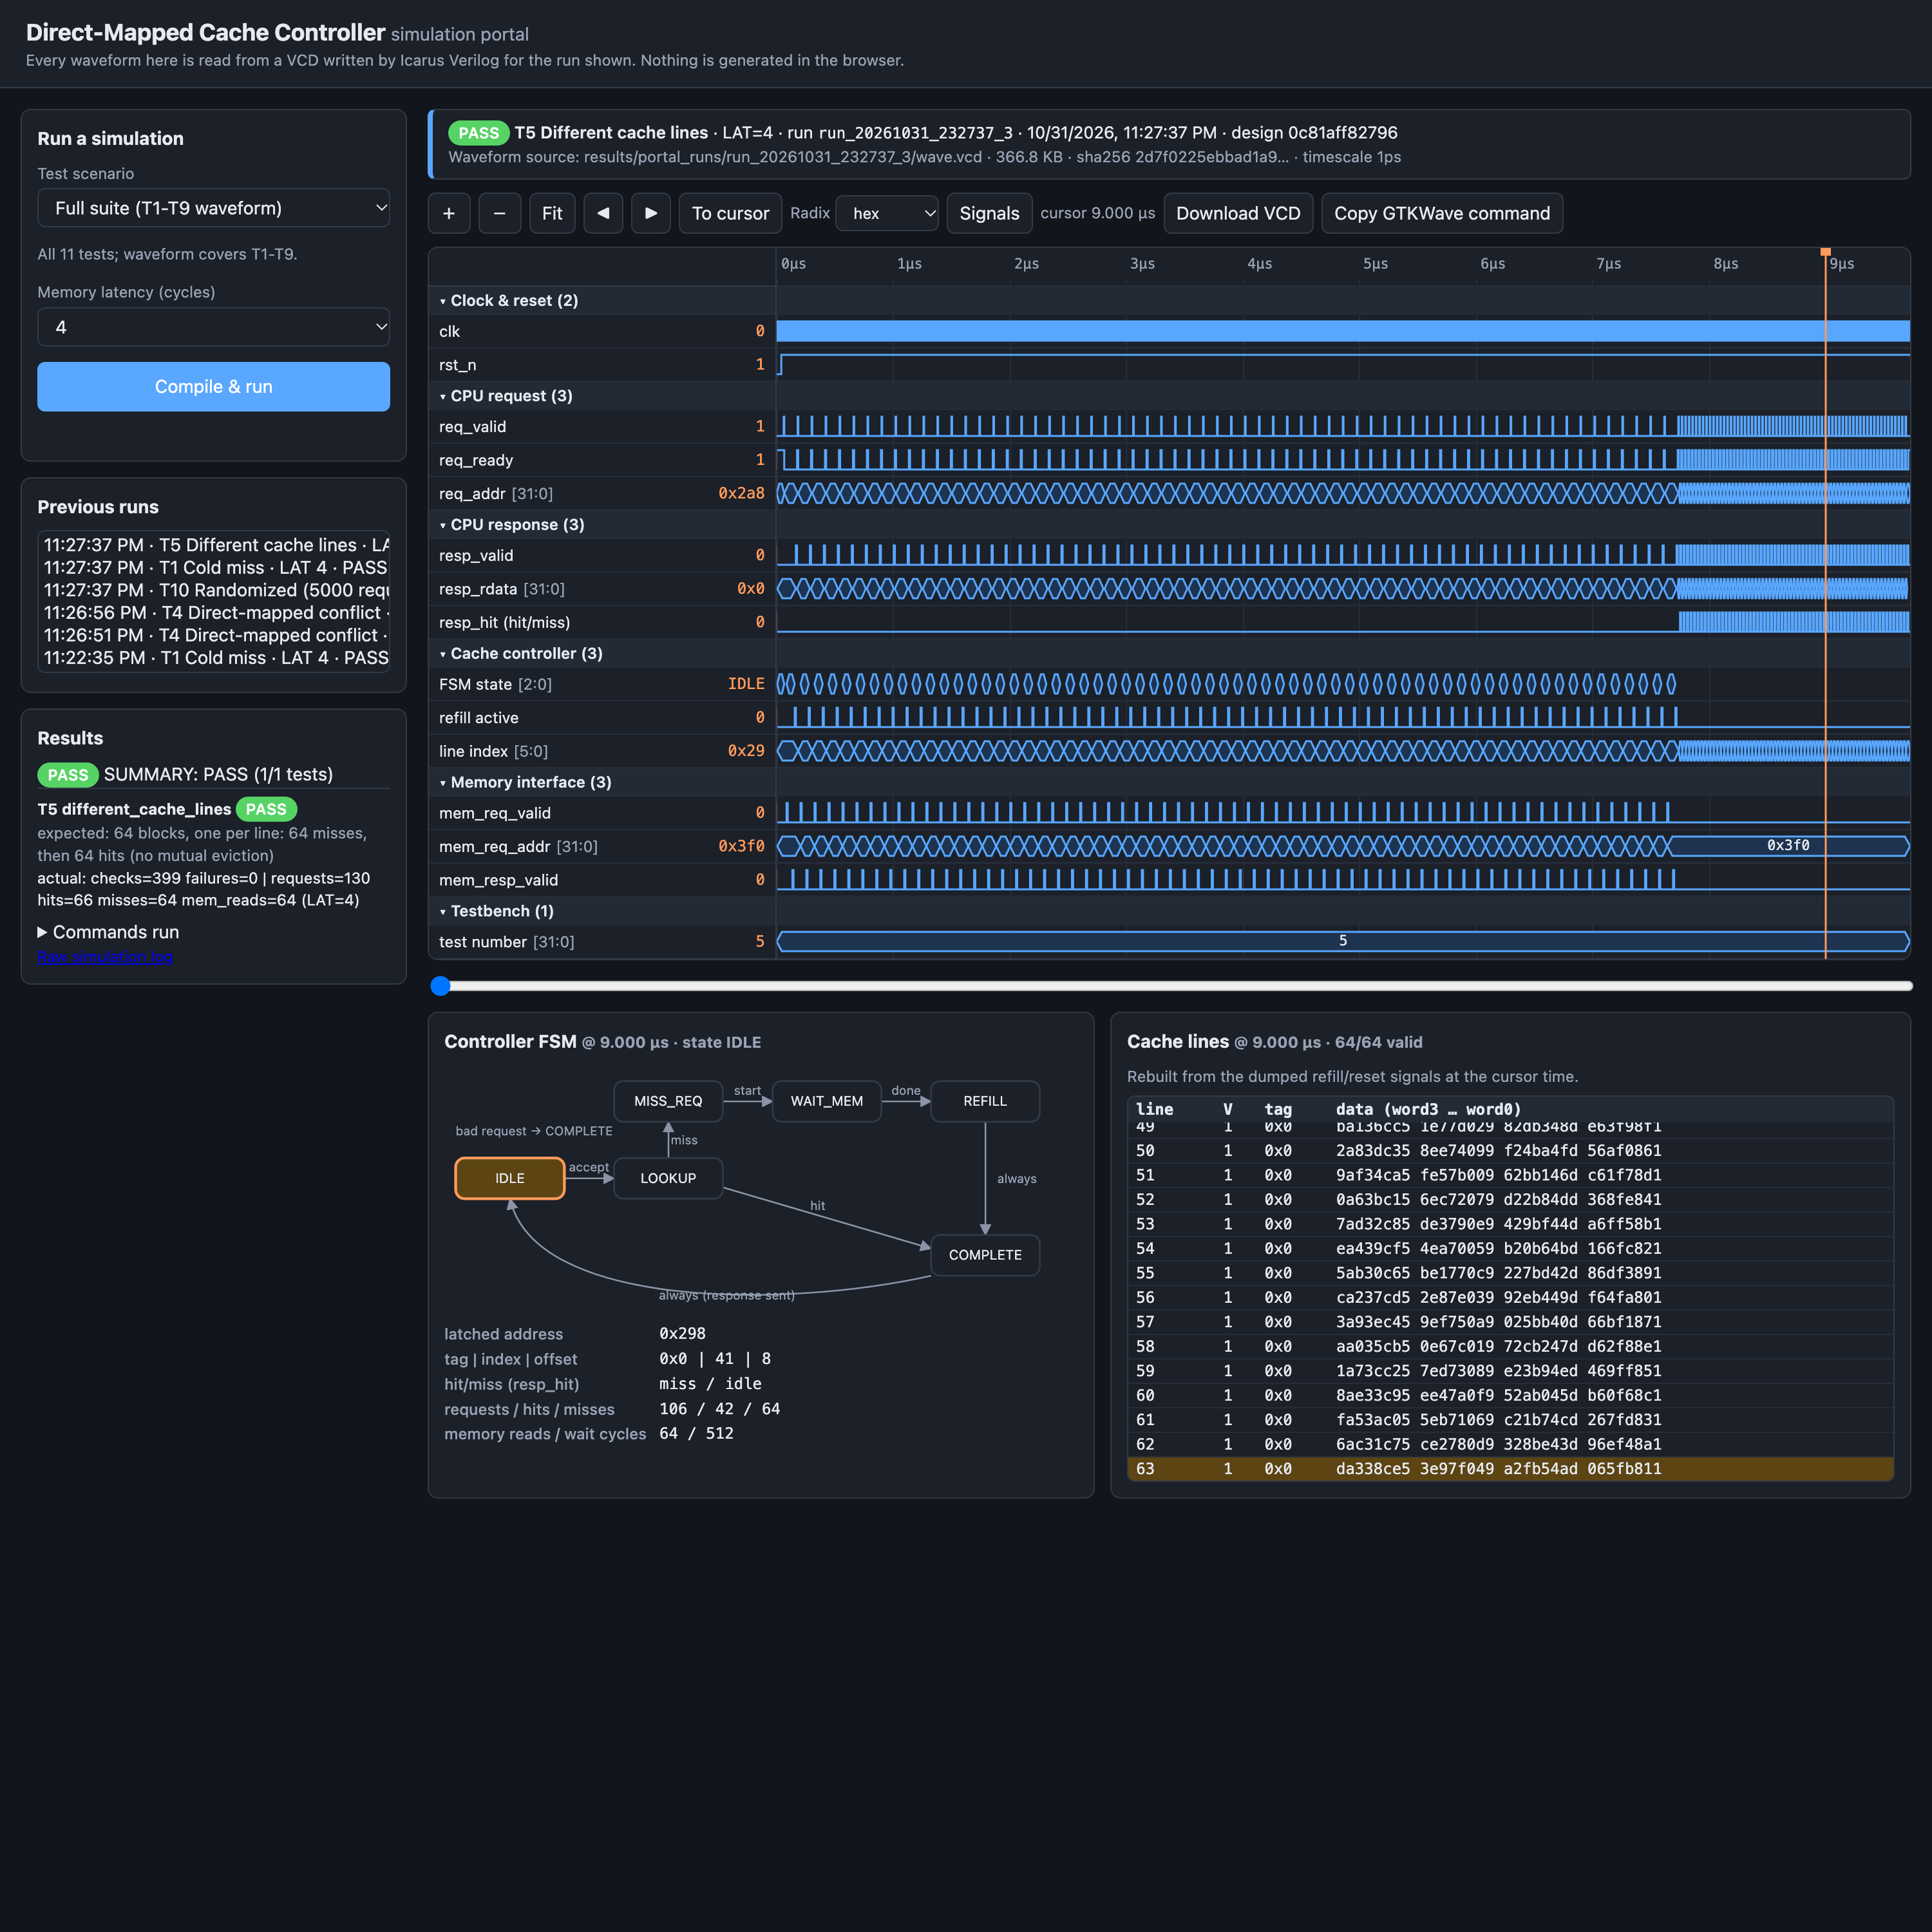
\includegraphics[width=0.66\textwidth]{portal_cache_lines.png}
\caption{Test~5 (64 different lines) near its end: the cache-line table shows many valid lines with their tags and data at the cursor time.}\label{fig:p-lines}
\end{figure*}

\begin{figure*}[t]
\centering
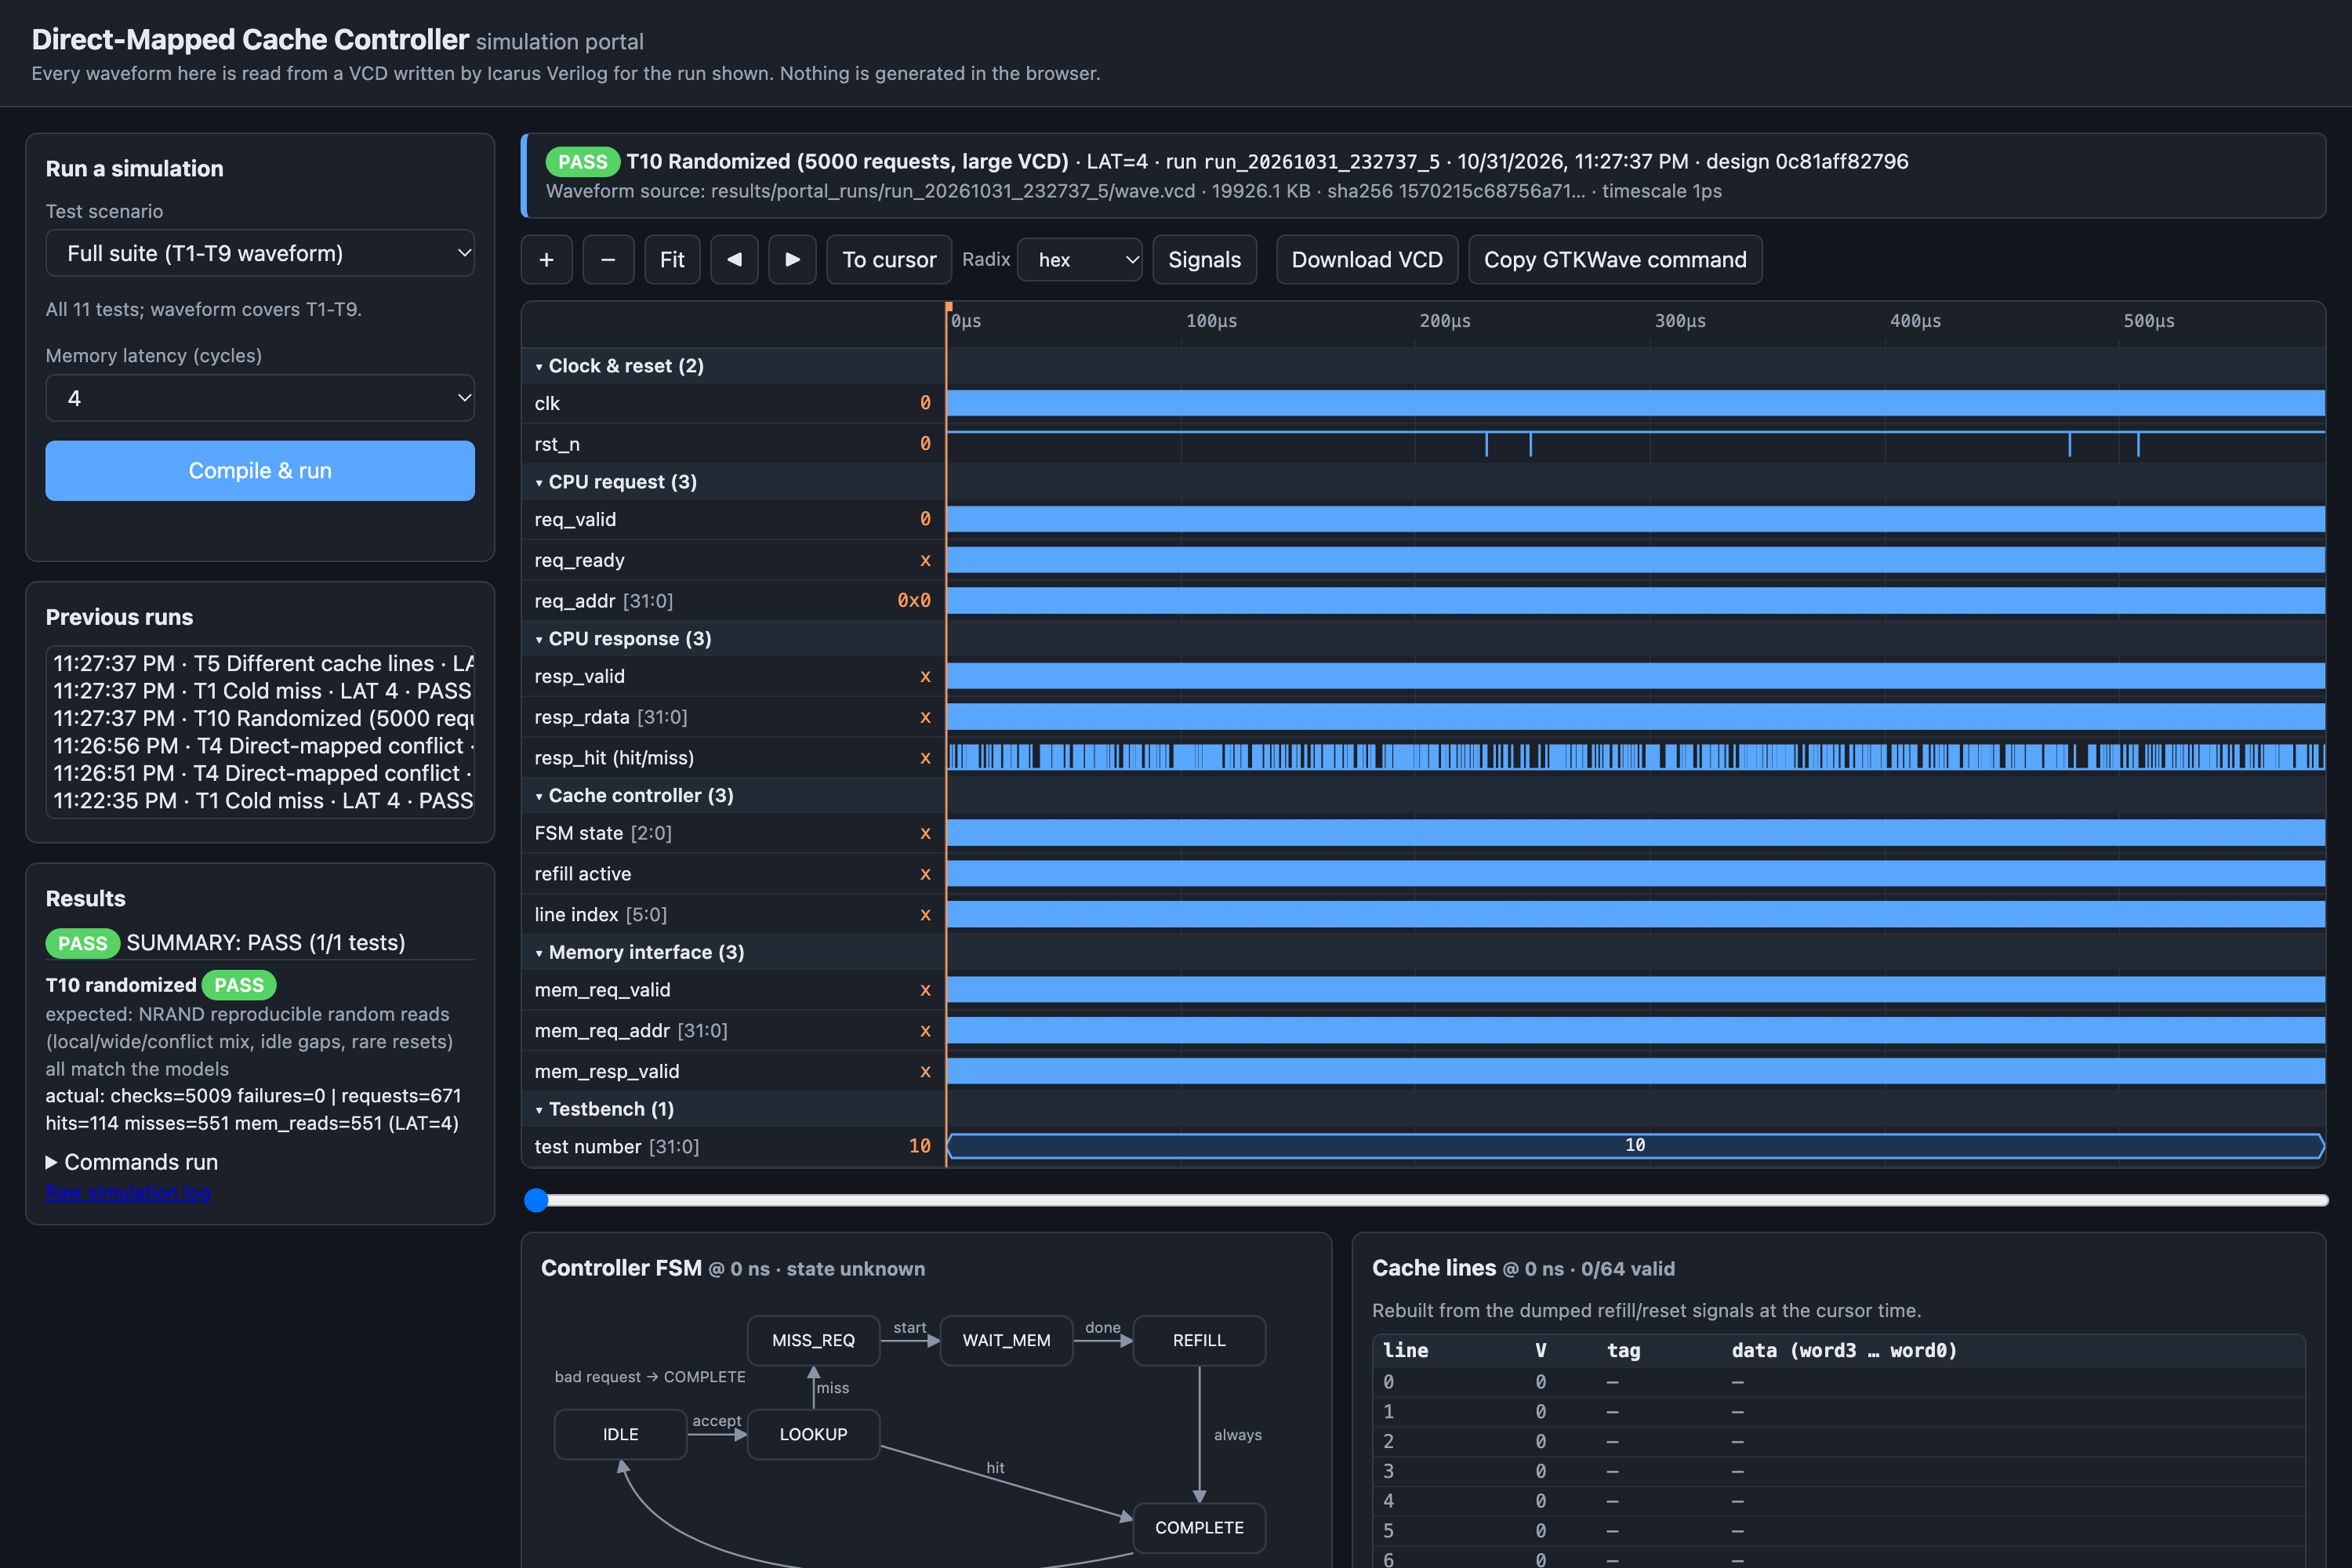
\includegraphics[width=0.8\textwidth]{portal_large.png}
\caption{The 5000-request random run (about 20~MB VCD) displayed in full: dense regions are reduced to the first and last change per pixel; zooming shows every transition.}\label{fig:p-large}
\end{figure*}

\subsection{Cache contents from dumped signals}
A VCD does not contain the contents of memory arrays. To show cache lines honestly, the backend rebuilds them \emph{only from signals that are in the VCD}:
\begin{itemize}
\item A line is written on the first clock edge after \code{refill_en} rises, using the dumped \code{q_index}, \code{q_tag} and \code{refill_block}.
\item All valid bits clear on a clock edge where \code{rst_n} is low.
\end{itemize}
This follows the RTL exactly. The write lands one cycle after \code{refill_en} rises, which is why Fig.~\ref{fig:p-zoom} shows an empty table at the instant the FSM is in REFILL.

\subsection{Handling large files}
The browser never receives a whole VCD. It asks for the visible time window of the selected signals; the backend keeps only the signals the viewer needs and answers from a sorted index. If a window contains more changes than pixels, only the first and last change per pixel column are returned and the row is marked dense. This keeps the page responsive for the 20~MB run in Fig.~\ref{fig:p-large}.

\subsection{Safety}
No command text, path or file name comes from the browser. Scenario and latency are checked against fixed lists, and anything else is rejected with an HTTP error. Commands run without a shell, in the project directory, with timeouts and size-limited output. Run identifiers must match a strict pattern \emph{and} belong to the server's own list; static files are served only from the portal directory; request bodies over 1~KB are refused.

\subsection{Evidence that every displayed waveform is real}
A verification script (\texttt{verify\_portal.py}) launches runs through the same code path as the portal and checks:
\begin{enumerate}
\item the VCD header is from Icarus Verilog and its SHA-256 matches the run record;
\item the portal's indexed values equal an independent re-parse of the VCD at 400 random times for all 30 signals (0 mismatches in all five runs checked, including the full suite);
\item the VCD's counters and the number of \code{resp_valid} pulses equal the numbers that the simulator itself printed in its log;
\item every reconstructed cache line matches the memory image;
\item the downloaded VCD is byte-identical to the file on disk; and
\item unapproved scenarios, latencies, malformed or oversized JSON, path traversal and unknown run identifiers are rejected.
\end{enumerate}
All checks pass.

%=====================================================================
\section{Overall Project Flow}\label{sec:flow}
\begin{figure*}[t]
\centering
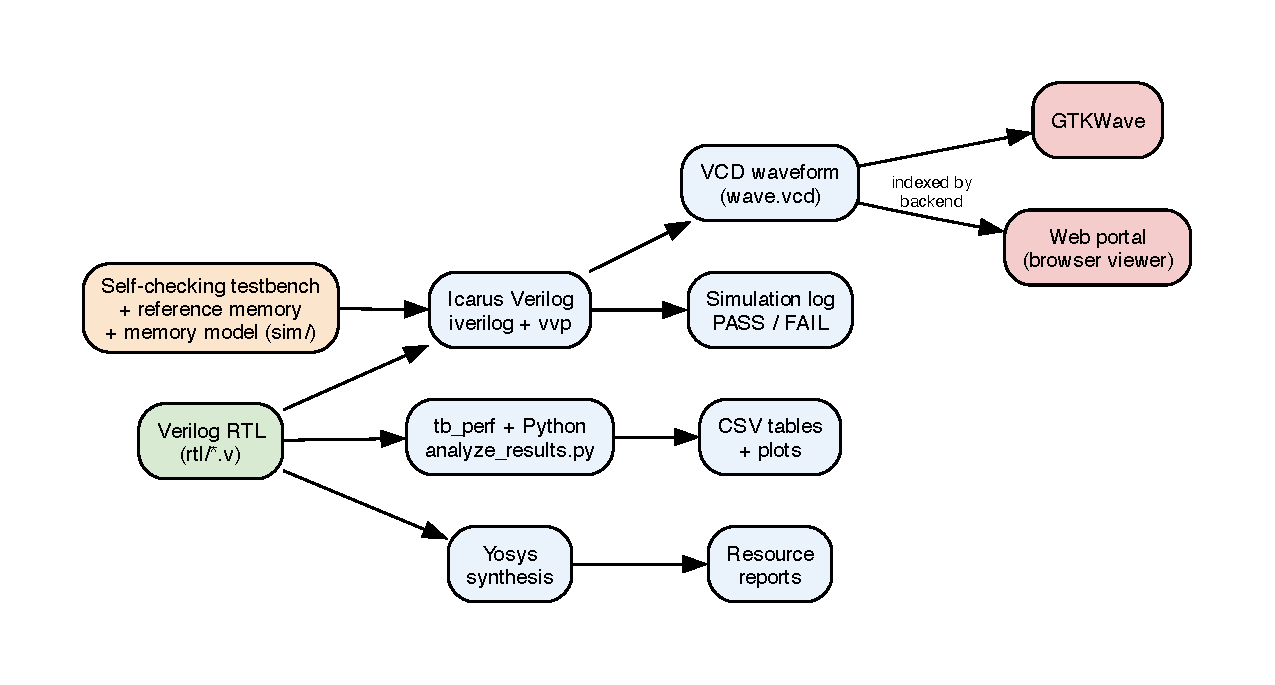
\includegraphics[width=0.95\textwidth]{toolflow.pdf}
\caption{Tool flow: RTL and testbench go through Icarus Verilog to a VCD and a log; the VCD feeds GTKWave and the portal; Python analyzes performance; Yosys estimates resources.}\label{fig:flow2}
\end{figure*}

The work followed eight phases: (1) environment setup; (2) architecture and interface specification; (3) RTL and unit tests; (4) memory model and first end-to-end simulation; (5) full self-checking verification; (6) performance measurement; (7) synthesis; (8) documentation, diagrams and the portal. Each phase ended with a pass check before the next began. Everything is reproducible with a single command per step: \code{make sim}, \code{make perf}, \code{make synth}, \code{make portal}, \code{make verify-portal}, or \code{make all} for the complete flow.

%=====================================================================
\section{Limitations and Future Work}
\begin{itemize}
\item The cache is read-only and blocking, with one request outstanding and 32-bit word-aligned accesses.
\item The memory model is always ready when idle, so memory back-pressure is untested.
\item Workloads are synthetic; cold-start statistics include compulsory misses.
\item Synthesis numbers are estimates, block RAM is under-used, and no timing analysis was done.
\item The portal runs only the listed scenarios (by design) and indexes 30 signals; cache contents are reconstructed, not dumped.
\end{itemize}
\emph{Future work:} write-through with write-allocate and byte enables; sweeps of capacity and block size; a 2-way set-associative comparison to remove conflict misses; optional statistics counters; fewer, wider RAM blocks; back-pressure tests; place-and-route timing; and traces from real programs.

%=====================================================================
\section{Conclusion}
A parameterized, synthesizable direct-mapped cache controller was designed, verified and analyzed using only software tools. Simulation confirms the derived equations: hit time of 2 cycles, miss penalty of $L+5$ cycles, and AMAT $=2+m(L+5)$ with no double counting. Measured miss rates agree with simple analytical models for repeated, sequential, conflicting, random and hot-region access. The testbench was shown to detect injected faults, and the interactive portal lets a reader inspect the real waveform, FSM state and cache contents for any scenario while keeping the original VCD for GTKWave. All results are from simulation and synthesis; no physical hardware validation was performed.

%\balance
\begin{thebibliography}{99}
\bibitem{hennessy2017} J. L. Hennessy and D. A. Patterson, \emph{Computer Architecture: A Quantitative Approach}, 6th ed. Morgan Kaufmann, 2017.
\bibitem{patterson2020} D. A. Patterson and J. L. Hennessy, \emph{Computer Organization and Design: The Hardware/Software Interface, RISC-V Edition}, 2nd ed. Morgan Kaufmann, 2020.
\bibitem{smith1982} A. J. Smith, ``Cache memories,'' \emph{ACM Computing Surveys}, vol.~14, no.~3, pp. 473--530, 1982.
\bibitem{hill1988} M. D. Hill, ``A case for direct-mapped caches,'' \emph{Computer}, vol.~21, no.~12, pp. 25--40, 1988.
\bibitem{jouppi1990} N. P. Jouppi, ``Improving direct-mapped cache performance by the addition of a small fully-associative cache and prefetch buffers,'' in \emph{Proc. 17th Int. Symp. Computer Architecture (ISCA)}, 1990, pp. 364--373.
\bibitem{wulf1995} W. A. Wulf and S. A. McKee, ``Hitting the memory wall: Implications of the obvious,'' \emph{ACM SIGARCH Computer Architecture News}, vol.~23, no.~1, pp. 20--24, 1995.
\bibitem{demillo1978} R. A. DeMillo, R. J. Lipton, and F. G. Sayward, ``Hints on test data selection: Help for the practicing programmer,'' \emph{Computer}, vol.~11, no.~4, pp. 34--41, 1978.
\bibitem{verilog2005} \emph{IEEE Standard for Verilog Hardware Description Language}, IEEE Std 1364-2005, 2006.
\bibitem{iverilog} S. Williams, ``Icarus Verilog,'' open-source Verilog simulator. [Online]. Available: \url{https://steveicarus.github.io/iverilog/}
\bibitem{yosys} C. Wolf, ``Yosys Open SYnthesis Suite,'' open-source synthesis framework. [Online]. Available: \url{https://yosyshq.net/yosys/}
\bibitem{gtkwave} ``GTKWave,'' open-source waveform viewer. [Online]. Available: \url{https://gtkwave.sourceforge.net/}
\end{thebibliography}

\end{document}
